\subsection{\texorpdfstring{以 \(\mu\) 为基的测度的特征刻画}{以 mu 为基的测度的特征刻画}}

定理 2（Lebesgue--Nikodym）. --- 设 \(\mu\) 和 \(\nu\) 是 T 上的两个正测度。下列性质等价：

\begin{enumerate}
\def\labelenumi{\arabic{enumi})}
\item
  \(\nu\) 是以 \(\mu\) 为基的测度。
\item
  每个局部 \(\mu\) -可忽略集都是局部 \(\nu\) -可忽略的。
\item
  每个 \(\mu\) -可忽略紧集都是 \(\nu\) -可忽略的。
\end{enumerate}

明显地，1) 蕴涵 2)（命题 3 的推论 1），且 2) 蕴涵 3)。我们将证明 3) 蕴涵 1)。首先注意，若条件 3) 满足，则每个普遍可测且局部 \(\mu\) -可忽略的集 A 都是局部 \(\nu\) -可忽略的；因为 \(\nu^{\bullet}(\mathrm{A}) = \sup \nu(\mathrm{K})\) ，其中 K 取遍含于 A 中的紧集所成之集（ \(\S 1\) , No.~3, 命题 10, a) 及 Ch. IV, \(\S 4\) , No.~6, 定理 4 的推论 2）。接下来，我们建立两个引理。

引理 2. --- 设 \(\alpha\) 是 T 上的一个有界正测度，\(\beta\) 是 T 上的一个实测度，满足 \(|\beta| \leqslant M\alpha\) ，其中 M 是一个正常数。则存在一个实函数 \(u\) ，它是 \(\alpha\) -可积的，使得 \(\beta = u \cdot \alpha\) 。

设 \(g\) 是空间 \(\mathcal{L}_{\mathbf{R}}^{2}(\mathrm{T},\alpha)\) 的一个元素；\(g\) 是 \(\beta\) -可测的，且 \(\int^{\bullet}|g|^2 d|\beta| \leqslant \mathrm{M}\int^{\bullet}|g|^2 d\alpha < +\infty\) 。因此函数 \(g\) 属于 \(\mathcal{L}^2 (\mathrm{T},|\beta|)\) ，而且也属于 \(\mathcal{L}^1 (\mathrm{T},|\beta|)\) ，因为 \(\beta\) 是有界的。由 Cauchy-Schwarz 不等式，

\[
| \beta (g) | ^ {2} \leqslant \left(\int | g | d | \beta |\right) ^ {2} \leqslant \left(\int d | \beta |\right) \left(\int | g | ^ {2} d | \beta |\right) \leqslant \mathrm{M} ^ {2} \alpha (1) \alpha (| g | ^ {2}).
\]

于是映射 \(g \mapsto \beta(g)\) 是 \(\mathcal{L}^2(\mathrm{T},\alpha)\) 上的一个连续线性形式。由于与 \(\mathcal{L}^2(\mathrm{T},\alpha)\) 相伴的 Hausdorff 空间是 Hilbert 空间，故存在（TVS, Ch. V, §1, No.~7, 定理 3）一个实函数 \(u \in \mathcal{L}^2(\mathrm{T},\alpha)\) （因而也属于 \(\mathcal{L}^1(\mathrm{T},\alpha)\) ），使得 \(\beta(g) = \alpha(ug)\) 对每个 \(g \in \mathcal{L}^2(\mathrm{T},\alpha)\) 都成立。把这个关系式应用于 \(g \in \mathcal{K}(\mathrm{T})\) ，即见 \(\beta = u\cdot \alpha\) 。

引理 3. --- 设正测度 \(\nu\) 使得每个 \(\mu\) -可忽略紧集都是 \(\nu\) -可忽略的。用 \(\mathfrak{K}\) 表示由具有下列性质的紧子集 \(K\) （\(T\) 中的）组成的集：

\begin{enumerate}
\def\labelenumi{(\arabic{enumi})}
\setcounter{enumi}{10}
\tightlist
\item
  存在一个常数 \(M \geqslant 0\) ，使得 \(\varphi_{K} \cdot \nu \leqslant M \varphi_{K} \cdot \mu\) 。此时集 K 在 T 中是 \(\mu\) -稠密的。
\end{enumerate}

若 K 满足 (11)，且 A 是含于 K 中的 Borel 集，则由命题 8 立即得出 \(\varphi_{\mathrm{A}} \cdot \nu \leqslant \mathrm{M}\varphi_{\mathrm{A}} \cdot \mu\) ；由此推出，K 与 \(K'\) （\(\mathfrak{K}\) 的两个元素）之并属于 \(\mathfrak{K}\) ，因为 \(\varphi_{\mathrm{K} \cup \mathrm{K}'} = \varphi_{\mathrm{K}} + \varphi_{\mathrm{A}}\) ，其中 \(\mathrm{A} = \mathrm{K}' \cap \mathbb{C}\mathrm{K}\) 。为建立引理，只须证明每个使 \(\mu(\mathrm{L}) > 0\) 的紧集 L 都包含一个紧集 \(\mathrm{K} \in \mathfrak{K}\) ，使得 \(\mu(\mathrm{K}) > 0\) （Ch. IV, §5, No.~8, 命题 12）。选取数 \(\mathrm{M} > \nu(\mathrm{L}) / \mu(\mathrm{L})\) ，并对有界正测度 \(\alpha = \varphi_{\mathrm{L}} \cdot (\nu + \mathrm{M}\mu)\) 与测度 \(\beta = \varphi_{\mathrm{L}} \cdot (\nu - \mathrm{M}\mu)\) 应用引理 1。如有必要，把函数 \(u\) （使 \(\beta = u \cdot \alpha\) 者）换成一个与它 \(\alpha\) -几乎处处相等的函数，就可以假设 \(u\) 是普遍可测的（§3, No.~4, 命题 7）且在 L 之外为零。由 \(t \in \mathrm{T}\) （使 \(u(t) < 0\) 者）组成的集 H 含于 L，它不可能是 \(\mu\) -可忽略的；因为否则它将是 \(\nu\) -可忽略的（由定理 2 证明开头的注记），从而是 \(\alpha\) -可忽略的，于是将有 \(\beta(\mathrm{L}) > 0\) ，这与 M 的选取相矛盾。设 K 是含于 H 中的一个紧集，使得 \(\mu(\mathrm{K}) > 0\) ；让我们证明 \(\mathrm{K} \in \mathfrak{K}\) ，这就将建立引理。由命题 8，

\[
\varphi_ {\mathrm{K}} \cdot (\nu - \mathrm{M} \mu) = \varphi_ {\mathrm{K}} \cdot \beta = \varphi_ {\mathrm{K}} \cdot (u \cdot \alpha) = (\varphi_ {\mathrm{K}} u) \cdot \alpha .
\]

函数 \(\varphi_{\mathbf{K}}u\) 是负的，因此确实有 \(\varphi_{\mathbf{K}}\cdot \nu \leqslant \mathrm{M}\varphi_{\mathbf{K}}\cdot \mu\) 。

现在来完成定理 2 的证明。假设条件 3) 成立，并按引理 3 那样定义 \(\mathfrak{K}\) 。设 \((\mathrm{K}_{\alpha})_{\alpha \in \mathbf{A}}\) 是 \(\mathfrak{K}\) 中两两不相交元素组成的一个局部可数族，使得集 \(\mathrm{N} = \mathrm{T} - \bigcup_{\alpha \in \mathbf{A}} \mathrm{K}_{\alpha}\) 是局部 \(\mu\) -可忽略的（Ch. IV, §5, No.~9, 命题 14）；由于族 \((\mathrm{K}_{\alpha})\) 是局部可数的，N 是普遍可测的，从而是局部 \(\nu\) -可忽略的。置 \(\mu_{\alpha} = \varphi_{\mathrm{K}_{\alpha}} \cdot \mu\) ，\(\nu_{\alpha} = \varphi_{\mathrm{K}_{\alpha}} \cdot \nu\) ；由于诸函数 \(\varphi_{\mathrm{K}_{\alpha}}\) 构成一个局部可数族，其和关于 \(\mu\) 与关于 \(\nu\) 都局部几乎处处等于 1 ，命题 6 蕴涵 \(\mu = \sum_{\alpha \in \mathbf{A}} \mu_{\alpha}\) ，\(\nu = \sum_{\alpha \in \mathbf{A}} \nu_{\alpha}\) 。另一方面，由 \(\mathfrak{K}\) 的定义，对每个 \(\alpha\) 存在常数 \(\mathrm{M}_{\alpha}\) ，使得 \(\nu_{\alpha} \leqslant \mathrm{M}_{\alpha} \mu_{\alpha}\) ；于是引理 2 蕴涵存在一个函数 \(g_{\alpha}\) （可以假设它在 \(\mathrm{K}_{\alpha}\) 之外为零且是正的）（命题 3 的推论 3），使得 \(\nu_{\alpha} = g_{\alpha} \cdot \mu_{\alpha}\) 。因此（No.~4, 命题 8）

\[
\nu_ {\alpha} = g _ {\alpha} \cdot \mu_ {\alpha} = g _ {\alpha} \cdot (\varphi_ {\mathrm{K} _ {\alpha}} \cdot \mu) = (g _ {\alpha} \varphi_ {\mathrm{K} _ {\alpha}}) \cdot \mu = g _ {\alpha} \cdot \mu .
\]

置 \(g = \sum_{\alpha \in A} g_{\alpha}\) ；由于族 \((g_{\alpha})\) 是局部可数的且族 \((\nu_{\alpha})\) 是可和的，命题 6 蕴涵 \(g\) 是局部 \(\mu\) -可积的，且 \(\nu = g \cdot \mu\) ，这就建立了定理。

推论 1. --- 设 N 是由以 \(\mu\) 为基的正测度组成的一个集，它有一个上确界 \(\nu\) （在 \(\mathcal{M}(\mathrm{T})\) 中）；则 \(\nu\) 是以 \(\mu\) 为基的测度。

命题 2 的推论允许化归到 N 是递增有向集的情形。于是，对每个局部 \(\mu\) -可忽略集 A ，依 §1, No.~4 的命题 11，有

\[
\nu^ {\bullet} (\mathrm{A}) = \sup _ {\lambda \in \mathcal {N}} \lambda^ {\bullet} (\mathrm{A}) = 0.
\]

因此定理 2 蕴涵 \(\nu\) 是以 \(\mu\) 为基的测度。

推论 2. --- 设 \(\nu\) 是 T 上的一个实测度。为使 \(\nu\) 属于由 \(\mu\) （在完全格序空间 \(\mathcal{M}(\mathrm{T})\) 中，Ch. II, §1, No.~5）生成的带，必须且只须 \(\nu\) 是以 \(\mu\) 为基的测度。

考虑 \(\nu^{+}\) 和 \(\nu^{-}\) ，立即化归到正测度 \(\nu\) 的情形（No.~2, 命题 2 的推论）。于是置 \(\nu_{n} = \inf(n\mu, \nu)\) ；\(\nu\) 属于由 \(\mu\) 生成的带当且仅当 \(\nu = \sup_{n} \nu_{n}\) （Ch. II, §1,

No.~5, 命题 6 的推论）。现在 \(\nu_{n}\) 被 \(n\mu\) 优超，故由定理 2 它是以 \(\mu\) 为基的测度；于是关系式 \(\nu = \sup_{n} \nu_{n}\) 蕴涵 \(\nu\) 是

以 \(\mu\) 为基的测度（推论 1）。反之，设 \(\nu\) 是以 \(\mu\) 为基的测度：\(\nu = g \cdot \mu\) ，其中 \(g\) 是局部 \(\mu\) -可积的正函数。此时 \(\nu_n = \inf(g, n) \cdot \mu\) （命题 2 的推论），且由 Lebesgue 定理（Ch. IV, §4, No.~3, 命题 4）立即得出 \(\nu = \sup_{n} \nu_n\) 。

推论 3. --- 设 \(\theta\) 是一个复测度；则存在一个普遍可测函数 \(v\) ，满足 \(|v| = 1\) ，使得 \(\theta = v \cdot |\theta|\) ，\(|\theta| = \overline{v} \cdot \theta\) 。

写 \(\theta = \theta_{1} - \theta_{2} + i(\theta_{3} - \theta_{4})\) ，其中 \(\theta_{1} = (\mathcal{R}\theta)^{+}\) ，\(\theta_{2} = (\mathcal{R}\theta)^{-}\) ，\(\theta_{3} = (\mathcal{I}\theta)^{+}\) ，\(\theta_{4} = (\mathcal{I}\theta)^{-}\) ；正测度 \(\theta_{i} (i = 1, 2, 3, 4)\) 被 \(|\theta|\) 优超（Ch. III, §1, No.~6, 公式 (17)），故由定理 2 都是以 \(|\theta|\) 为基的测度。由此推出，存在一个局部 \(|\theta|\) -可积函数 v ，使得 \(\theta = v \cdot |\theta|\) 。于是命题 2 给出关系 \(|\theta| = |v| \cdot |\theta|\) ，它蕴涵 \(|v| = 1\) 局部 \(|\theta|\) -几乎处处成立（命题 3 的推论 2）。最后，由命题 8，\(\overline{v} \cdot \theta = (v\overline{v}) \cdot |\theta| = |\theta|\) 。由于函数 v 只在一个局部 \(|\theta|\) -可忽略函数的范围内有定义，可以假设 v 是普遍可测的（§3, No.~4, 命题 7）且处处 \(|v| = 1\) 。

评注. --- 1) 设 \(\lambda\) 是一个正测度，\(v\) 是一个 \(\lambda\) -可测函数，满足 \(|v| = 1\) 局部 \(\lambda\) -几乎处处成立（这蕴涵 \(v\) 是局部 \(\lambda\) -可积的），并且 \(\theta = v \cdot \lambda\) 。命题 2 立即表明 \(\lambda = |\theta|\) ；换句话说，前一陈述的性质刻画了正测度 \(|\theta|\) 。

\begin{enumerate}
\def\labelenumi{\arabic{enumi})}
\setcounter{enumi}{1}
\tightlist
\item
  若 \(|\theta| \leqslant a\mu\) ，其中 \(\mu\) 是一个正测度且 \(a\) 是一个数 \(\geqslant 0\) ，则 \(\theta\) 是以 \(\mu\) 为基的测度。
\end{enumerate}

推论 4. --- 设 \(\rho\) 和 \(\theta\) 是两个复测度。为使存在一个局部 \(\theta\) -可积函数 \(u\) ，使得 \(\rho = u \cdot \theta\) ，必须且只须每个 \(\theta\) -可忽略紧集都是 \(\rho\) -可忽略的。

该条件显然是必要的。反之，设每个 \(\theta\) -可忽略紧集都是 \(\rho\) -可忽略的；定理 2 蕴涵存在一个局部 \(|\theta|\) -可积函数 g ，使得 \(|\rho| = g \cdot |\theta|\) 。另一方面，推论 3 蕴涵存在一个函数 \(v_{1}\) （相应地，\(v_{2}\) ），其绝对值为 1 且对测度 \(|\rho|\) （相应地，\(\theta\) ）可测，使得 \(\rho = v_{1} \cdot |\rho|\) （相应地，\(|\theta| = \overline{v}_{2} \cdot \theta\) ）。于是，由命题 8，\(\rho = u \cdot \theta\) ，其中 \(u = v_{1}g\overline{v}_{2}\) 。

推论 5. --- 设 \(\mu\) 和 \(\nu\) 是 T 上的两个正测度。定理 2 的条件 1)、2)、3) 也等价于下列条件：

\begin{enumerate}
\def\labelenumi{\arabic{enumi})}
\setcounter{enumi}{3}
\item
  对每个 \(\nu\) -可积数值函数 \(f \geqslant 0\) 及每个数 \(\varepsilon > 0\) ，存在一个 \(\delta > 0\) ，使得关系 \(0 \leqslant h \leqslant f\) 与 \(\int^{*} h d\mu \leqslant \delta\) 蕴涵 \(\int^{*} h d\nu < \varepsilon\) 。
\item
  对每个函数 \(g \in \mathcal{K}_{+}(\mathrm{T})\) 及每个数 \(\varepsilon > 0\) ，存在一个 \(\delta > 0\) ，使得对每个 \(h \in \mathcal{K}_{+}(\mathrm{T})\) （被 \(g\) 优超且满足 \(\int h d\mu \leqslant \delta\) 者），有 \(\int h d\nu \leqslant \varepsilon\) 。
\item
  对每个紧集 \(\mathbf{K} \subset \mathbf{T}\) 及每个数 \(\varepsilon > 0\) ，存在一个 \(\delta > 0\) ，使得关系 \(\mathbf{A} \subset \mathbf{K}\) 与 \(\mu^{*}(\mathbf{A}) \leqslant \delta\) 蕴涵 \(\nu^{*}(\mathbf{A}) \leqslant \varepsilon\) 。蕴涵关系 4) \(\Rightarrow 6) \Rightarrow 3)\) 是明显的。
\end{enumerate}

设存在一个有限函数 \(k \geqslant 0\) ，普遍可测且局部 \(\mu\) -可积，使得 \(\nu = k \cdot \mu\) ，让我们证明条件 4) 满足。设 f 是一个 \(\nu\) -可积函数 \(\geqslant 0\) ，并设 \(\varepsilon > 0\) 。对每个整数 \(n \geqslant 0\) ，设 \(A_{n}\) 是由 \(t \in T\) （使 \(k(t) \geqslant n\) 者）组成的集。诸函数 \(f\varphi_{A_{n}}\) 构成一个递减序列，被 f 优超且逐点趋于 0 ，因此存在一个 N ，使得 \(\int f\varphi_{A_{N}} d\nu \leqslant \varepsilon/2\) （Ch. IV, §4, No.~3, 命题 4）。若 h 是 T 上满足 \(0 \leqslant h \leqslant f\) 与 \(\int^{*} h d\mu \leqslant \varepsilon/2N\) 的函数，则

\[
\begin{array}{r l} & {\nu^ {*} (h) \leqslant \nu^ {*} (h \varphi_ {\mathrm {A_ {N}}}) + \nu^ {*} \big (h (1 - \varphi_ {\mathrm {A_ {N}}}) \big)} \\ & {\quad \leqslant \nu^ {*} (f \varphi_ {\mathrm {A_ {N}}}) + \mu^ {*} \big (h (1 - \varphi_ {\mathrm {A_ {N}}}) k \big)} \\ & {\quad \leqslant \frac {\varepsilon}{2} + \mathrm{N} \mu^ {*} (h) \leqslant \varepsilon .} \end{array}
\]

于是我们证明了条件 4) 与 6) 等价于定理 2 的诸条件。

明显地，4) 蕴涵 5)。最后，若条件 5) 满足，则 \(\nu\) 属于由 \(\mu\) 生成的带（Ch. II, §2, No.~2, 命题 5），从而以 \(\mu\) 为基（推论 2）。

概说. --- 对每个 \(\dot{f} \in \mathrm{L}_{\mathrm{loc}}^{1}(\mathrm{T}, \mu; \mathbf{R})\) ，置 \(\varphi(\dot{f}) = f \cdot \mu\) ，其中 \(f \in \dot{f}\) ；映射 \(\varphi\) 是线性的、递增的且单射的（命题 3 的推论 2），它在 \(\mathcal{M}(\mathrm{T})\) 中的像是由 \(\mu\) 生成的带 B（定理 2 的推论 2）。于是映射 \(\varphi\) 允许把 \(\mathrm{L}_{\mathrm{loc}}^{1}(\mathrm{T},\mu;\mathbf{R})\) 等同于 T 上的一个实测度空间；由于诸空间 \(\mathrm{L}_{\mathbf{R}}^{p}(\mathrm{T},\mu)\) 都是 \(\mathrm{L}_{\mathrm{loc}}^{1}(\mathrm{T},\mu;\mathbf{R})\) 的子空间，它们也可以等同于 \(\mathcal{M}(\mathrm{T})\) 的子空间。对复值函数与复测度有类似的考虑。注意，上面考虑的映射 \(\varphi\) 是 \(L_{loc}^{1}\) 与 B 的序向量空间结构之间的同构，但显然不是这些空间的拓扑向量空间结构之间的同构。

\pandocbounded{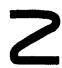
\includegraphics[keepaspectratio]{images/part002_ab1a0807.jpg}}

由于完全格序空间中的每个带本身都是完全格序空间（Ch. II, §1, No.~5），可见空间 \(L_{loc}^{1}\) 是完全格序的；但值得回忆的是，在 \(L_{loc}^{1}\) 中，一个由等价类组成的不可数族 \((\dot{f}_{\alpha})\) 的上确界不一定等同于诸函数 \(f_{\alpha}\) 的上包络的类。然而我们已看到，对于一个递增序列 \((f_{n})\) （由局部 \(\mu\) -可积函数组成），若其上包络 f 是局部 \(\mu\) -可积的，则 \(f \cdot \mu\) 是测度序列 \((f_{n} \cdot \mu)\) 在 \(\mathcal{M}(T)\) 中的上确界（命题 6 的推论）。

下面是定理 2 的推论 3 的一个有趣推论：

命题 9. --- 设 \(\theta\) 是一个有界复测度；为使 \(\theta\) 是正测度，必须且只须 \(\| \theta \| = \theta(1)\) 。

该条件显然是必要的。反之，设 \(\|\theta\|=\int d\theta\) ，并用 v 表示一个绝对值为 1 的 \(|\theta|\) -可测函数，使得 \(\theta=v\cdot|\theta|\) 。由于 \(\|\theta\|=\int d|\theta|\) （Ch. IV, §4, No.~7, 命题 12）且 \(\int d\theta=\int v\cdot d|\theta|\) （定理 1），假设蕴涵 \(\int(1-v)d|\theta|=0\) ，从而 \(\int\mathcal{R}(1-v)d|\theta|=0\) 。于是函数 \(\mathcal{R}(1-v)\) 是正的，故几乎处处为零，这蕴涵 v=1 几乎处处成立，证明完毕。

\subsection{等价测度}

命题 10. --- 设 \(\mu\) 和 \(\nu\) 是 T 上的两个正测度。下列条件等价：

\begin{enumerate}
\def\labelenumi{\alph{enumi})}
\item
  局部可忽略集对 \(\mu\) 和对 \(\nu\) 是相同的。
\item
  由 \(\mu\) 和 \(\nu\) 在 \(\mathcal{M}(\mathrm{T})\) 中生成的带是相同的。
\item
  有 \(\nu = g \cdot \mu\) ，其中 \(g\) 是局部 \(\mu\) -可积的，且 \(g(t) > 0\) 关于 \(\mu\) 局部几乎处处成立。
\end{enumerate}

条件 a) 与 b) 依 No.~5 的定理 2 的推论 2 而等价。若它们成立，则 \(\nu = g \cdot \mu\) 且 \(\mu = h \cdot \nu\) ，其中 \(g\) （相应地，\(h\) ）对 \(\mu\) （相应地，\(\nu\) ）是正的且局部可积的。因此（No.~4, 命题 8）\(hg\) 是局部 \(\mu\) -可积的，且 \(\mu = (hg) \cdot \mu\) 。由此推出（No.~3, 命题 3 的推论 2）\(hg\) 关于 \(\mu\) 局部几乎处处等于 1 ，从而 \(g(t) > 0\) 与 \(h(t) = 1/g(t)\) 关于 \(\mu\) 局部几乎处处成立。反之，设 \(\nu = g \cdot \mu\) ，其中 \(g(t) > 0\) 关于 \(\mu\) 局部几乎处处成立；

由于 \((1/g)g\) 局部几乎处处有定义且是局部 \(\mu\) -可积的，1/g 是局部 \(\nu\) -可积的，且 \((1/g)\cdot\nu=\mu\) （No.~4, 命题 8）。

定义 3. --- 局部紧空间 T 上的两个复测度 \(\theta, \theta'\) 称为等价的，如果测度 \(|\theta|\) 和 \(|\theta'|\) 满足命题 10 的条件 a)、b)、c)。

因此，为使 \(\theta\) 和 \(\theta'\) 等价，必须且只须 \(|\theta|\) 和 \(|\theta'|\) 等价。

注. --- 若 \(\mu\) 和 \(\nu\) 是两个等价的正测度，则定义在 T 上、取值于任意拓扑空间 G 中的可测函数对 \(\mu\) 和对 \(\nu\) 是相同的，这由 No.~3 的命题 4 立即得出。

命题 11. --- 设 \(\mu\) 是 T 上的一个正测度。若 T 在无穷远处可数，则存在一个连续函数 \(h\) ，使得 \(h(t) > 0\) 对所有 \(t \in \mathrm{T}\) 成立，且使测度 \(\nu = h \cdot \mu\) （与 \(\mu\) 等价）是有界的。

设 \((\mathrm{K}_{n})\) 是构成 T 的覆盖的一个紧集序列，且对每个 n ，设 \(f_{n}\) 是 \(\mathcal{K}(\mathrm{T})\) 中的一个函数，满足 \(0 \leqslant f_{n} \leqslant 1\) 且 \(f_{n}(t) = 1\) 在 \(\mathrm{K}_{n}\) 上成立（Ch. III, §1, No.~2, 引理 1）。设 \((a_{n})\) 是一个数 \textgreater{} 0 的序列，使得 \(\sum_{n} a_{n} < +\infty\) ；于是级数 \(h = \sum_{n} a_{n} f_{n}\) 在 T 中正规收敛，因而 h 是 T 上的连续函数，使得 \(h(t) > 0\) 对所有 \(t \in \mathrm{T}\) 成立，这是按构造方式得到的。置 \(\nu = h \cdot \mu\) ，我们就有（命题 3 及 Ch. IV, §1, No.~3, 命题 13）

\[
\nu^ {*} (1) = \int^ {*} h d \mu \leqslant \sum_ {n} a _ {n} \int f _ {n} d \mu .
\]

例如，取 \(a_{n} = 2^{-n}\left(\int f_{n}d\mu\right)^{-1}\) 当 \(\int f_n d\mu > 1\) 时，否则取 \(a_{n} = 2^{-n}\) ，我们就有了 \(\sum_{n}a_{n} < +\infty\) 且 \(\nu^{*}(1) < +\infty\) ，这就证明了命题。

命题 12. --- 设 \((\mu_n)\) 是 T 上的一个有界正测度序列；则存在 T 上的一个有界正测度 \(\mu\) ，使得关系 \(\mu^*(\mathrm{N}) = 0\) 等价于 \(\langle \mu_n^*(\mathrm{N}) = 0 \text{ 对每个 } n \rangle\) ；每个测度 \(\mu_n\) 都以 \(\mu\) 为基。此外，若 \(\mu'\) 是另一个具有此性质的 T 上的正测度，则 \(\mu\) 和 \(\mu'\) 等价。

陈述的最后一部分由定义 3 立即得出。为证明 \(\mu\) 的存在性，可以限于 \(\mu_n \neq 0\) （对每个 \(n\) ）的情形；于是测度族 \(\mu_n / 2^n \| \mu_n \|\) 在 \(\mathcal{M}(\mathrm{T})\) 中是可和的，其和 \(\mu\) 满足 \(\| \mu \| \leqslant 1\) 。此外，由于 \(\mu_n \leqslant 2^n \| \mu_n \| \cdot \mu\) ，关系 \(\mu(\mathrm{N}) = 0\) 蕴涵 \(\mu_n(\mathrm{N}) = 0\) 对一切 \(n\) 成立；反之，若 \(\mathrm{N}\) 是一个对所有 \(\mu_n\) 都可忽略的集，则它对 \(\mu\) 是局部可忽略的（§2, No.~2, 命题 1 的推论 2），从而由于 \(\mu\) 有界，它是 \(\mu\) -可忽略的（§1, No.~2, 命题 7 的推论 2）。

\subsection{互奇异测度}

对 T 上的两个实测度 \(\rho,\sigma\) ，回忆一下，称 \(\rho\) 和 \(\sigma\) 是互奇异的，如果 \(\inf(|\rho|,|\sigma|)=0\) 在 \(\mathcal{M}(\mathrm{T})\) 中成立（Ch. II, §1, No.~1）。已知与一个给定测度互奇异的诸实测度构成一个带（Ch. II, §1, No.~5, 定理 1）。这个定义可以立即推广到复测度的情形。

定义 4. --- 称 T 上的一个复测度 \(\theta\) 集中于 T 的一个子集 M 上，或称 M 承载 \(\theta\) ，如果 \(\mathbb{C}M\) 对 \(\theta\) 是局部可忽略的。

集 M 承载 \(\theta\) 当且仅当它承载 \(|\theta|\) 。说 M 承载 \(\theta\) ，等价于说 M 是 \(\theta\) -可测的且 \(\theta = \varphi_{M} \cdot \theta\) 。若 \(\theta\) 集中于 M，则每个以 \(|\theta|\) 为基的测度都集中于 M。

命题 13. --- 为使 T 上的两个复测度 \(\rho\) 和 \(\sigma\) 互奇异，必须且只须在 T 中存在两个不相交的集 R 和 S ，使得 \(\rho\) 集中于 R 且 \(\sigma\) 集中于 S；可以取 R 和 S 为普遍可测的。

置 \(\mu = |\rho|\) ，\(\nu = |\sigma|\) ，\(\lambda = \mu + \nu\) ；由于 \(\mu\) 和 \(\nu\) 被 \(\lambda\) 优超，存在两个局部 \(\lambda\) -可积函数 u 和 v （依 §3, No.~4, 命题 7 可设它们是普遍可测的），使得 \(\mu = u \cdot \lambda\) ，\(\nu = v \cdot \lambda\) 。于是

\[
\inf (| \rho |, | \sigma |) = \inf (\mu , \nu) = \inf (u, v) \cdot \lambda
\]

（No.~2, 命题 2 的推论）。设 A （相应地，B ）是由 \(t \in \mathbf{T}\) （使 \(u(t) > 0\) 且 \(v(t) = 0\) （相应地，\(u(t) = 0\) 且 \(v(t) > 0\) ）者）组成的集。若 \(\rho\) 和 \(\sigma\) 互奇异，则 \(\inf(u, v) = 0\) 局部 \(\lambda\) -几乎处处成立（No.~3, 命题 3 的推论 2），于是不相交的普遍可测集 A 和 B 分别承载 \(\mu\) 和 \(\nu\) 。反之，设 \(\mu\) 和 \(\nu\) 分别由不相交的集 R 和 S 承载；\(\varphi_{\mathrm{R}}\) 对测度 \(\mu = u \cdot \lambda\) 可测，且 \(\mu = \varphi_{\mathrm{R}} \cdot \mu\) 。由 No.~4 的命题 8，函数 \(u' = u\varphi_{\mathrm{R}}\) 是 \(\lambda\) -可测的，且 \(\mu = u' \cdot \lambda\) 。类似地，若 \(v' = v\varphi_{\mathrm{S}}\) ，则 \(\nu = v' \cdot \lambda\) ；注意到 \(\inf(u', v') = 0\) （No.~2, 命题 2 的推论），即得结论。

推论 1. --- 对 T 上的每个实测度 \(\nu\) ，存在两个不相交的集 M,N ，分别承载 \(\nu^{+}\) 和 \(\nu^{-}\) 。

\pandocbounded{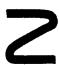
\includegraphics[keepaspectratio]{images/part002_61ad429f.jpg}}

必须注意不要把测度 \(\nu\) 的支集的概念与 \(\nu\) 所集中的集的概念相混淆。\(\nu\) 的支集 S 是承载 \(\nu\) 的最小闭集（Ch. III, §2, No.~2, 命题 2 及 Ch. IV, §2, No.~2, 命题 5）。然而，可能存在 S 的与 S 不同却承载 \(\nu\) 的子集。更一般地，可以有 \(\inf(\mu,\nu)=0\) ，对两个具有相同支集的正测度 \(\mu\) 和 \(\nu\) 而言（习题 5）。

还要注意，承载 \(\nu\) 的诸集之交是由 \(t \in T\) （使 \(|\nu|(\{t\}) > 0\) 者）组成的点的集，它可以是空集（例如 Lebesgue 测度的情形）；因此，一般不存在承载 \(\nu\) 的最小集。

推论 2. --- 设 \(\rho\) 和 \(\sigma\) 是两个互奇异的复测度，\(\rho'\) 和 \(\sigma'\) 是两个复测度，分别具有关于 \(\rho\) 和 \(\sigma\) 的密度；则 \(\rho'\) 和 \(\sigma'\) 互奇异。

推论 3. --- 设 \(\rho\) 和 \(\sigma\) 是两个互奇异的复测度；则 \(|\rho + \sigma| = |\rho| + |\sigma|\) 。

用 v （相应地，w ）表示一个绝对值为 1 的普遍可测函数，使得 \(\rho = v \cdot |\rho|\) （相应地，\(\sigma = w \cdot |\sigma|\) ）（定理 2 的推论 3），并用 A 表示一个承载 \(\rho\) 的普遍可测集，使得 B = C A 承载 \(\sigma\) （命题 13）；则也有 \(\rho + \sigma = (v\varphi_{\mathrm{A}} + w\varphi_{\mathrm{B}}) \cdot (|\rho| + |\sigma|)\) 。由于函数 \(v\varphi_{A} + w\varphi_{B}\) 的绝对值等于 1 ，推论由命题 2 得出。

定理 3（Lebesgue）. --- T 上的每个复测度 \(\theta\) 都可以以一种且仅一种方式写成 \(\theta = g \cdot \mu + \theta'\) 的形式，其中 \(g\) 是局部 \(\mu\) -可积的，\(\theta'\) 是一个与 \(\mu\) 互奇异的测度。此时 \(|\theta| = |g| \cdot \mu + |\theta'|\) 。

当 \(\theta\) 是正的时，这由 F. Riesz 定理（Ch. II, §1, No.~5, 定理 1）（应用于 T 上的实测度所组成的完全格序空间 \(\mathcal{M}(T)\) 以及 \(\mu\) 在此空间中生成的带，并注意到 No.~5 的定理 2 的推论 2）立即得出；此外，此时 \(\theta'\) 和 \(g \cdot \mu\) 都是正的，这蕴涵 \(g\) 局部 \(\mu\) -几乎处处为正（命题 3 的推论 3）。为处理 \(\theta\) 不是正的情形，置 \(\nu = |\theta|\) ，\(\nu = f \cdot \mu + \nu'\) （其中 \(f\) 是正的，且 \(\nu'\) 与 \(\mu\) 互奇异），并置 \(\theta = v \cdot \nu\) ，其中 \(v\) 是一个绝对值为 1 的普遍可测函数（定理 2 的推论 3）。于是我们有（命题 8）\(\theta = g \cdot \mu + \theta'\) ，其中 \(g = vf\) （从而 \(|g| = f\) ）且 \(\theta' = v \cdot \nu'\) （从而依命题 2 有 \(|\theta'| = \nu'\) ）；测度 \(\theta'\) 与 \(\mu\) 依命题 13 的推论 2 互奇异。只须再建立分解的唯一性。于是，设 \(\theta = g \cdot \mu + \theta' = g_1 \cdot \mu + \theta'_1\) ，其中 \(\theta'\) 和 \(\theta'_1\) 都与 \(\mu\) 互奇异；\(|\theta' - \theta'_1|\) 被 \(|\theta'| + |\theta'_1|\) 优超，因此 \(\theta' - \theta'_1\) 与 \(\mu\) 互奇异，从而也与 \((g_1 - g) \cdot \mu\) 互奇异。于是关系 \(\theta' - \theta'_1 = (g_1 - g) \cdot \mu\) 蕴涵两个成员都为零，这就证明了唯一性。

回忆（No.~5, 定理 2 及概说），空间 \(\mathrm{L}_{\mathrm{loc}}^{1}(\mathrm{T},\mu;\mathbf{C})\) 可以（借助映射 \(g\mapsto g\cdot\mu\) ）等同于 \(\mathcal{M}_{\mathbf{C}}(\mathrm{T})\) 的一个子空间。在这一约定下，定理 3 取下列形式：

推论. --- 存在一个投影子 \(p\) （由空间 \(\mathcal{M}_{\mathbf{C}}(\mathrm{T})\) 到空间 \(\mathrm{L}_{\mathrm{loc}}^{1}(\mathrm{T},\mu ;\mathbf{C})\) 上的），其核 \(\overline{p}^{1}(0)\) 是与 \(\mu\) 互奇异的复测度所组成的集，使得

\[
| \theta | = | p (\theta) | + | \theta - p (\theta) |, \quad p (| \theta |) = | p (\theta) |
\]

对每个复测度 \(\theta\) 都成立。

若把 p 限制在有界测度所成之集上，就得到一个投影子 \(p^{1}\) （由空间 \(\mathcal{M}_{\mathbf{C}}^{1}(\mathrm{T})\) 到空间 \(\mathrm{L}_{\mathbf{C}}^{1}(\mathrm{T},\mu)\) 上的）；关系 \(\|\theta\|=|\theta|(1)\) 蕴涵 \(\|\theta\|=\|p^{1}(\theta)\|+\|\theta-p^{1}(\theta)\|\) 对每个有界复测度 \(\theta\) 成立。

\subsection{\texorpdfstring{应用：I. \(L^{p}\) 空间的对偶}{应用：I. L to the p 空间的对偶}}

我们在这里只处理实空间 \(\mathbf{L}^p\) 的情形。

回忆一下，两个数 \(p, q\) （满足 \(1 \leqslant p \leqslant +\infty\) ，\(1 \leqslant q \leqslant +\infty\) ，\(1/p + 1/q = 1\) 者）称为共轭指数（Ch. IV, §6, No.~4）。每个函数 \(g \in \mathcal{L}^q\) 定义一个连续线性形式 \(\theta_g\) （\(L to the p\) 上的），它是由线性形式 \(f \mapsto \int fg d\mu\) （\(\mathcal{L}^p\) 上的）出发过渡到商而得到的，并且有 \(N_q(g) = \| \theta_g \|\) （Ch. IV, §6, No.~4, 命题 3 的推论）。通过过渡到商，我们就从映射 \(g \mapsto \theta_g\) 得到一个等距线性映射 \(\varphi\) ，把 \(L^q\) 映入对偶 \((L to the p)'\) （\(L to the p\) 的）。我们将证明，对 \(1 \leqslant p < +\infty\) ，\(\varphi\) 把 \(L^q\) 映到 \((L to the p)'\) 上，因而今后我们可以把 Banach 空间 \(L^q\) 与 Banach 空间 \((L to the p)'\) 借助同构 \(\varphi\) 等同起来。用另一种方式陈述：

定理 4. --- 设 p 和 q 是满足 \(1 \leqslant p < +\infty\) 的两个共轭指数。\(\mathcal{L}^{p}(\mathrm{T}, \mu)\) 上的每个连续线性形式都是 \(f \mapsto \int fg d\mu\) 型的，其中 g 是 \(\mathcal{L}^{q}(\mathrm{T}, \mu)\) 中的一个函数，它的类在 \(L^{q}\) 中是适定的。

设 \(\theta\) 是 \(\mathcal{L}^p\) 上的一个连续线性形式；于是，存在一个数 \(a \geqslant 0\) ，使得 \(|\theta(f)| \leqslant a \cdot \mathrm{N}_p(f)\) 对每个函数 \(f \in \mathcal{L}^p\) 成立。考察 \(\theta\) 在具有紧支集的连续函数所组成的空间 \(\mathcal{K}(\mathrm{T})\) 上的限制：对 T 的每个紧子集 K 以及每个函数 \(f \in \mathcal{K}(\mathrm{T}, \mathrm{K})\) （支集含于 K 中的连续函数所组成的空间），有 \(\mathrm{N}_p(f) \leqslant (\mu(\mathrm{K}))^{1/p} \| f \|\) ；因此在 \(\mathcal{K}(\mathrm{T}, \mathrm{K})\) 上由 \(\mathcal{L}^p\) 的拓扑诱导的拓扑比一致收敛拓扑粗，从而 \(\theta\) 在每个 \(\mathcal{K}(\mathrm{T}, \mathrm{K})\) 上的限制对后一拓扑是连续的。这意味着 \(\theta\) 在 \(\mathcal{K}(\mathrm{T})\) 上的限制是一个实测度 \(\nu\) （Ch. III, §1, No.~3, 定义 2）。

我们来证明 \(|\nu|(|f|) \leqslant a \cdot \mathrm{N}_{p}(f)\) 对 \(\mathcal{K}(\mathrm{T})\) 中的每个函数 f 成立。只须对 \(f \geqslant 0\) 证明此公式。现在，对每个函数 \(\psi\) （\(\mathcal{K}(\mathrm{T})\) 中满足 \(|\psi| \leqslant f\) 者），我们有

\[
| \nu (\psi) | \leqslant a \cdot \mathrm{N} _ {p} (\psi) \leqslant a \cdot \mathrm{N} _ {p} (f);
\]

我们的断言由 Ch. III, §1, No.~6 公式 (12) 给出的测度绝对值的表达式得出。关系 \(|\nu|(|f|) \leqslant a(\mu(|f|^p))^{1/p}\) 通过过渡到下包络，立即推广到 \(f\) 是一个紧集的特征函数的情形，然后它蕴涵每个 \(\mu\) -可忽略的紧集都是 \(\nu\) -可忽略的，从而 \(\nu\) 是一个以 \(\mu\) 为基的测度（No.~5, 定理 2）。

于是，存在一个局部 \(\mu\) -可积的正函数 \(h_1\) ，使得 \(|\nu|(f) = \int fh_1 d\mu\) 对每个函数 \(f \in \mathcal{K}(\mathrm{T})\) 成立。我们来证明，\(h_1\) 局部几乎处处等于 \(\mathcal{L}^q\) 中的一个函数。若函数 \(f \geqslant 0\) 属于 \(\mathcal{K}(\mathrm{T})\) 且满足 \(\mathrm{N}_p(f) \leqslant 1\) ，则 \(\int fh_1 d\mu = |\nu|(f) \leqslant a\) 。对每个连续映射 \(f_0\) （由 \(\mathrm{T}\) 到 {[}0,1{]} 中且具有紧支集的），我们因此有 \(\sup \int (f_0 h_1) f d\mu \leqslant a\) ，其中 \(f\) 跑遍函数 \(\geqslant 0\) （\(\mathcal{K}(\mathrm{T})\) 中满足 \(\mathrm{N}_p(f) \leqslant 1\) 者）所成之集。由此，借助 Chap. IV, §6, No.~4 的公式 (11)，可以推出 \(\mathrm{N}_q(f_0 h_1) \leqslant a\) 。从而 \(\sup_{\mathrm{K}} \mathrm{N}_q (\varphi_{\mathrm{K}} h_1) \leqslant a\) ，其中 \(\mathrm{K}\) 跑遍 \(\mathrm{T}\) 的紧子集所成之集，这就证明了我们的断言（§1, 命题 9）。

设 v 是一个绝对值为 1 的普遍可测（实）函数，使得 \(\nu = v \cdot |\nu|\) （定理 2 的推论 3），并设 \(g = v h_{1}\) ；则 \(\nu = g \cdot \mu\) ，且 g 属于 \(L^{q}\) 。对每个函数 \(f \in \mathcal{K}(T)\) ，我们有 \(\theta(f) = \nu(f) = \int fg d\mu\) 。换言之，连续线性形式 \(\theta\) 和 \(\theta_{g}\) 在 \(\mathcal{K}(T)\) 上一致；因而它们在 \(L^{p}\) 上相等，因为 \(\mathcal{K}(T)\) 在 \(L^{p}\) 中稠密，这就完成了证明。

推论. --- 对满足 \(1 < p < +\infty\) 的每个数 p ，Banach 空间 \(L^{p}(T, \mu)\) 是自反的。

\pandocbounded{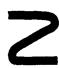
\includegraphics[keepaspectratio]{images/part002_5aba953c.jpg}}

一般地，\(L^{\infty}\) 的对偶不同构于 \(L^{1}\) ，因而 \(L^{1}\) 和 \(L^{\infty}\) 不是自反的（习题 10）。我们来刻画 \(L^{\infty}\) 上由线性形式 \(g \mapsto \int fg d\mu\) （\(L^{\infty}\) 上的，其中 \(g \in L^{1}\) ）过渡到商而产生的那些连续线性形式。

序向量空间 \(\mathrm{L}^{\infty}(\mathrm{T},\mu)\) （它是 \(\mathrm{L}_{\mathrm{loc}}^{1}(\mathrm{T},\mu)\) 的一个子空间）是完全格序的；因为，若 \((f_{\alpha})\) 是 \(L^{\infty}\) 中的正函数的一个族，其类所成之集 \((\dot{f}_{\alpha})\) 在 \(L^{\infty}\) 中有上界，则存在 \(a\geqslant0\) ，使得 \(\mathrm{N}_{\infty}(f_{\alpha})\leqslant a\) 对一切 \(\alpha\) 成立。由于 \(\mathrm{L}_{\mathrm{loc}}^{1}(\mathrm{T},\mu)\) 是完全格序的，族 \((\dot{f}_{\alpha})\) 有一个上确界 \(\dot{h}\) （在 \(\mathrm{L}_{\mathrm{loc}}^{1}(\mathrm{T},\mu)\) 中）；但由于 \(\dot{a}\geqslant\dot{f}_{\alpha}\) 对每个 \(\alpha\) 成立，我们有 \(\dot{h}\leqslant\dot{a}\) ，从而 \(\mathrm{N}_{\infty}(h)\leqslant a\) ，由此得到我们的断言。

命题 14. --- 为使一个正线性形式 \(\theta\) （\(\mathcal{L}^{\infty}\) 上的）是 \(f \mapsto \int fg d\mu\) 型的（其中 \(g \in \mathcal{L}^{1}\) ），必须且只须：对每个递增有向的正函数族 \((f_{\alpha})_{\alpha \in \mathrm{A}}\) （\(\mathcal{L}^{\infty}\) 中的），若其类所成之集 \((\dot{f}_{\alpha})_{\alpha \in \mathrm{A}}\) 在 \(\mathrm{L}^{\infty}\) 中有上界且在此空间中以 \(\dot{h}\) 为上确界，则有

\[
\theta (h) = \sup _ {\alpha \in \mathrm{A}} \theta (f _ {\alpha}).
\]

我们先证明条件是必要的。测度 \(h \cdot \mu\) 在 \(\mathcal{M}(\mathrm{T})\) 中是测度 \(f_{\alpha} \cdot \mu\) 所成之集的上确界（No.~5, 概说）；因此（Ch. II, §2, No.~2），对每个函数 \(\varphi \geqslant 0\) （\(\mathcal{K}(\mathrm{T})\) 中的），我们有 \(\int h\varphi d\mu = \sup_{\alpha \in \mathrm{A}} \int f_{\alpha}\varphi d\mu\) 。现在，若 \(a\) 是一个数 \(\geqslant 0\) ，使得 \(\mathrm{N}_{\infty}(f_{\alpha}) \leqslant a\) 对所有 \(\alpha \in \mathrm{A}\) 成立（这蕴涵 \(\mathrm{N}_{\infty}(h) \leqslant a\) ），则对每个 \(\varepsilon > 0\) ，存在一个 \(\varphi \in \mathcal{K}(\mathrm{T})\) ，满足 \(\varphi \geqslant 0\) 且 \(\mathrm{N}_1(g - \varphi) \leqslant \varepsilon\) ，由此我们推出 \(\int f_{\alpha}|g - \varphi| d\mu \leqslant a\varepsilon\) 对所有 \(\alpha \in \mathrm{A}\) 成立，以及 \(\int h|g - \varphi| d\mu \leqslant a\varepsilon\) 。由于 \(\sup_{\alpha \in \mathrm{A}} \int f_{\alpha}g d\mu \leqslant \int hg d\mu\) ，这就证明了这个不等式的两个成员相等。

为证明条件是充分的，我们将用到下列引理：

引理 4. --- \(1^{\circ}\) 设 \(f\) 是 \(\mathbf{T}\) 上的一个下半连续且有界的正函数。则它的类 \(\dot{f}\) （\(\mathbf{L}^{\infty}\) 中的）是类 \(\dot{\varphi}\) 所成之集的上确界，其中 \(\varphi\) 跑遍 \(\mathcal{K}(\mathbf{T})\) 中满足 \(0 \leqslant \varphi \leqslant f\) 的函数所成之集。

\(2^{\circ}\) 设 \(f\) 是 \(\mathbf{T}\) 上的一个可测且有界的正函数。则它的类 \(\dot{f}\) （\(\mathrm{L}^{\infty}\) 中的）是类 \(\dot{\psi}\) 所成之集的下确界，其中 \(\psi\) 跑遍 \(\mathbf{T}\) 上的下半连续且有界且 \(\geqslant f\) 的函数所成之集。

\(1^{\circ}\) 设 \(f'\) 是 \(\mathcal{L}^{\infty}\) 中的一个函数，使得 \(\dot{f}'\) 在 \(\mathrm{L}^{\infty}\) 中是类 \(\dot{\varphi}\) 所成之集的上确界，其中 \(\varphi\) 跑遍 \(\mathcal{K}(\mathrm{T})\) 中满足 \(0 \leqslant \varphi \leqslant f\) 的函数；显然 \(\dot{f}' \leqslant \dot{f}\) 。设 U 是 T 的一个相对紧开子集；对每个函数 \(h\) （\(\mathcal{K}(\mathrm{T})\) 中满足 \(0 \leqslant h \leqslant f\varphi_{\mathrm{U}}\) 者），依定义有 \(h(t) \leqslant f'(t)\) 局部几乎处处成立，因此 \(h(t) \leqslant f'(t)\varphi_{\mathrm{U}}(t)\) 几乎处处成立；由此推出 \(\int h d\mu \leqslant \int f'\varphi_{\mathrm{U}} d\mu\) 。然而，由于 \(f\varphi_{\mathrm{U}}\) 是下半连续的，有 \(\int f\varphi_{\mathrm{U}} d\mu = \sup \int h d\mu\) ，其中 \(h\) 跑遍 \(\mathcal{K}(\mathrm{T})\) 中满足 \(0 \leqslant h \leqslant f\varphi_{\mathrm{U}}\) 的函数所成之集（Ch. IV, §1, No.~1, 定义 1）；因此

\[
\int f \varphi_ {\mathrm{U}} d \mu \leqslant \int f ^ {\prime} \varphi_ {\mathrm{U}} d \mu ,
\]

而由于 \(f' \varphi_{\mathrm{U}} \leqslant f \varphi_{\mathrm{U}}\) 几乎处处成立，必然有 \(f \varphi_{\mathrm{U}} = f' \varphi_{\mathrm{U}}\) 几乎处处成立，从而 \(f = f'\) 局部几乎处处成立。

\(2^{\circ}\) 设 \(f'\) 是 \(\mathcal{L}^{\infty}\) 中的一个函数，使得 \(\dot{f}'\) 在 \(\mathrm{L}^{\infty}\) 中是由类 \(\dot{\psi}\) （\(\psi\) 为有界且 \(\geqslant f\) 的下半连续函数）组成的集的下确界；则 \(\dot{f}' \geqslant \dot{f}\) 。设 K 是 T 的一个紧子集；对每个下半连续且有界且 \(\geqslant f\varphi_{K}\) 的函数 h ，用 \(\overline{h}\) 表示在 K 上等于 h 且在 T - K 上等于 \(\|f\| + \|h\|\) 的函数。则 \(\overline{h}\) 是下半连续的且 \(\geqslant f\) ，因此依定义 \(\overline{h}(t) \geqslant f'(t)\) 局部几乎处处成立；由此推出 \(h(t) \geqslant f'(t)\varphi_{\mathrm{K}}(t)\) 几乎处处成立，从而 \(\int h d\mu \geqslant \int f'\varphi_{K} d\mu\) 。但 \(\int f\varphi_{K} d\mu = \inf \int h d\mu\) ，其中 h 跑遍下半连续且有界且 \(\geqslant f\varphi_{K}\) 的函数所成之集（Ch. IV, §1, No.~3, 定义 3）；因此

\[
\int f \varphi_ {\mathrm{K}} d \mu \geqslant \int f ^ {\prime} \varphi_ {\mathrm{K}} d \mu ,
\]

而由于 \(f\varphi_{\mathrm{K}} \leqslant f'\varphi_{\mathrm{K}}\) 几乎处处成立，必然有 \(f\varphi_{\mathrm{K}} = f'\varphi_{\mathrm{K}}\) 几乎处处成立，从而 \(f = f'\) 局部几乎处处成立。

引理既已证明，设 \(\theta\) 是 \(\mathcal{L}^{\infty}\) 上满足命题 14 陈述中条件的正线性形式。\(\theta\) 在空间 \(\mathcal{K}(\mathrm{T})\) 上的限制是一个正测度 \(\nu\) （\(\mathrm{T}\) 上的）。我们将证明，对每个正函数 \(f\in \mathcal{L}^{\infty}(\mathrm{T},\mu)\) ，有 \(\theta (f) = \nu^{*}(f)\) 。先设 \(f\) 是下半连续的（且有界）；由引理 4，\(\dot{f}\) 是类 \(\dot{\varphi}\) 的递增有向集的上确界，其中 \(\varphi\) 跑遍有向集 \(\Phi\) （由 \(\mathcal{K}(\mathrm{T})\) 中满足 \(0\leqslant \varphi \leqslant f\) 的函数组成）。由于依假设 \(\theta (f) = \sup_{\varphi \in \Phi}\theta (\varphi)\) ，且依定义 \(\nu^{*}(f) = \sup_{\varphi \in \Phi}\nu (\varphi)\) ，我们的断言在这一情形得证。其次，设 \(f\) 是 \(\mu\) -可测且有界的；则依定义 \(\nu^{*}(f) = \inf_{\psi \in \Psi}\nu^{*}(\psi)\) ，其中 \(\psi\) 跑遍递减有向集 \(\Psi\) （由下半连续且有界且 \(\geqslant f\) 的函数组成）。若 \(a\geqslant \| f\|\) ，则把陈述中的假设应用于函数 \(a - \psi\) （\(\psi \in \Psi\) 且 \(\psi \leqslant a\) 者）的类所组成的递增有向集，即依引理看出 \(\theta (f) = \inf_{\psi \in \Psi}\theta (\psi)\) ，因而确有 \(\theta (f) = \nu^{*}(f)\) 。特别地，对每个 \(\mu\) -可忽略的函数 \(f\geqslant 0\) ，有 \(\theta (f) = 0\) ，因此 \(\nu^{*}(f) = 0\) ，从而（No.~5, 定理 2）\(\nu\) 是一个以 \(\mu\) 为基的测度；此外，\(\nu^{*}(1) = \theta (1) < +\infty\) ，因而（定理 1 的推论）\(\nu = g\cdot \mu\) ，其中 \(g\in \mathcal{L}^1 (\mathrm{T},\mu)\) 。最后，由于每个 \(\mu\) -可测函数都是 \(\nu\) -可测的，每个正函数 \(f\in \mathcal{L}^{\infty}(\mathrm{T},\mu)\) 都是 \(\nu\) -可积的，且 \(\int fg d\mu = \nu^{*}(f) = \theta (f)\) ，这就完成了证明。

由命题 14 可以得出，\(\mathcal{L}^{\infty}\) 上 \(f\mapsto \int fg d\mu\) 型（其中 \(g\in \mathcal{L}^{1}\) ）的线性形式就是差 \(\theta_{1} - \theta_{2}\) ，其中 \(\theta_{1}\) 和 \(\theta_{2}\) 是满足命题 14 的条件的正线性形式。

\subsection{应用：II. 测度的函数}

设 \(\mu_1, \mu_2, \ldots, \mu_n\) 是 \(T\) 上的实测度，并设 \(u(x_1, \ldots, x_n)\) 是定义在 \(\mathbf{R}^n\) 上的一个有限数值函数，且是正齐次的，也就是说（Ch. I, §1, No.~1），满足

\[
u (\alpha x _ {1}, \ldots , \alpha x _ {n}) = \alpha u (x _ {1}, \ldots , x _ {n})\tag{12}
\]

对每个标量 \(\alpha \geqslant 0\) 。存在 T 上的正测度 \(\lambda\) ，使得 \(|\mu_i| \leqslant \lambda\) 对 \(1 \leqslant i \leqslant n\) 成立（例如和 \(\sum_{i=1}^{n} |\mu_i|\) ）。设 \(\lambda\) 和 \(\lambda'\) 是 T 上的两个这样的测度。可以写 \(\mu_i = f_i \cdot \lambda = f_i' \cdot \lambda'\) ，其中 \(f_i\) （相应地，\(f_i'\) ）对测度 \(\lambda\) （相应地，\(\lambda'\) ）是可测的且本性有界的（No.~5, 定理 2）。我们将建立下列结果：为使数值函数 \(u(f_1, \ldots, f_n)\) 对 \(\lambda\) 局部可积，必须且只须函数 \(u(f_1', \ldots, f_n')\) 对 \(\lambda'\) 局部可积，此时

\[
u (f _ {1}, \dots , f _ {n}) \cdot \lambda = u (f _ {1} ^ {\prime}, \dots , f _ {n} ^ {\prime}) \cdot \lambda^ {\prime}.
\]

由于 \(|\mu_i| \leqslant \inf(\lambda, \lambda')\) ，我们可以限于 \(\lambda \leqslant \lambda'\) 的情形。此时 \(\lambda = g \cdot \lambda'\) ，其中 \(g\) 是一个 \(\lambda'\) -可测函数，满足 \(0 \leqslant g \leqslant 1\) （No.~5, 定理 2）；由此（No.~4, 命题 8）得

\[
\mu_ {i} = f _ {i} \cdot (g \cdot \lambda^ {\prime}) = (f _ {i} g) \cdot \lambda^ {\prime};
\]

由此（No.~3, 命题 3 的推论 2）推出，\(f_{i}g\) 等于 \(f_{i}'\) （关于 \(\lambda'\) 局部几乎处处）。于是，由 (12)，

\[
u (f _ {1} ^ {\prime}, \dots , f _ {n} ^ {\prime}) = u (f _ {1} g, \dots , f _ {n} g) = u (f _ {1}, \dots , f _ {n}) g
\]

关于 \(\lambda'\) 局部几乎处处成立。为使 \(u(f_1', \ldots, f_n')\) 是局部 \(\lambda'\) -可积的，因此必须且只须 \(u(f_1, \ldots, f_n)g\) 对 \(\lambda'\) 局部可积，从而（No.~4, 命题 8）只须 \(u(f_1, \ldots, f_n)\) 对 \(\lambda\) 局部可积；此时（No.~4, 命题 8）

\[
u \left(f _ {1} ^ {\prime}, \dots , f _ {n} ^ {\prime}\right) \cdot \lambda^ {\prime} = \left(u \left(f _ {1}, \dots , f _ {n}\right) g\right) \cdot \lambda^ {\prime} = u \left(f _ {1}, \dots , f _ {n}\right) \cdot \lambda .
\]

于是，测度 \(u(f_{1},\ldots,f_{n})\cdot\lambda\) 只依赖于测度 \(\mu_{1},\ldots,\mu_{n}\) 和函数 u；它也记作 \(u(\mu_{1},\ldots,\mu_{n})\) 。因此，只要 u 是这样一个正齐次函数：对一个正测度 \(\lambda\) （它是所有 \(|\mu_{i}|\) 的上界）而言，\(u(f_{1},\ldots,f_{n})\) 是局部 \(\lambda\) -可积的（其中 \(f_{i}\) 表示 \(\mu_{i}\) 关于 \(\lambda\) 的密度），这个测度就有定义。注意，当 u 是正齐次且连续的函数时，这一条件是满足的：因为此时有

\[
\left| u \left(x _ {1}, \dots , x _ {n}\right) \right| \leqslant a \left(\left| x _ {1} \right| + \left| x _ {2} \right| + \dots + \left| x _ {n} \right|\right)
\]

（u 在 \((0,\ldots,0)\) 的一个充分小的邻域中有界），而且由于 \(u(f_{1},\ldots,f_{n})\) 是 \(\lambda\) -可测的（Ch. IV, §5, No.~3, 定理 1），根据可积性判别法（Ch. IV, §5, No.~6, 定理 5），它是局部 \(\lambda\) -可积的。

设 \(u_1, \ldots, u_p\) 是定义在 \(\mathbf{R}^n\) 上的正齐次数值函数，使得这 \(p\) 个函数 \(g_k = u_k(f_1, \ldots, f_n)\) （\(1 \leqslant k \leqslant p\) ）都是局部 \(\lambda\) -可积的。设 \(v\) 是定义在 \(\mathbf{R}^p\) 上的一个正齐次数值函数，使得 \(v(g_1, \ldots, g_p)\) 是局部 \(\lambda\) -可积的。置

\[
w (x _ {1}, \ldots , x _ {n}) = v \big (u _ {1} (x _ {1}, \ldots , x _ {n}), \ldots , u _ {p} (x _ {1}, \ldots , x _ {n}) \big).
\]

于是，函数 w 是正齐次的，\(w(f_{1}, \ldots, f_{n})\) 是局部 \(\lambda\) -可积的，且依定义，

\[
w \left(\mu_ {1}, \dots , \mu_ {n}\right) = v \left(u _ {1} \left(\mu_ {1}, \dots , \mu_ {n}\right), \dots , u _ {p} \left(\mu_ {1}, \dots , \mu_ {n}\right)\right).
\]

在函数 \(x^{+}\) ，\(x^{-}\) ，\(|x|\) ，\(x + y\) ，\(\inf(x, y)\) ，\(\sup(x, y)\) 的特殊情形，刚才所述程序所定义的测度分别与已记作 \(\mu^{+}\) ，\(\mu^{-}\) ，\(|\mu|\) ，\(\mu + \nu\) ，\(\inf(\mu, \nu)\) ，\(\sup(\mu, \nu)\) 的那些测度重合；这由 No.~2 的命题 2 的推论立即得出。若 \(\mu\) 和 \(\nu\) 是两个实测度，且 \(\theta = \mu + i\nu\) ，则 \(|\theta| = \sqrt{\mu^{2} + \nu^{2}}\) ；因为，设 \(\lambda\) 是一个测度 \(\geqslant 0\) ，它是 \(|\mu|\) 和 \(|\nu|\) 的一个上界，并设 f, g 是局部 \(\lambda\) -可积函数，使得 \(\mu = f \cdot \lambda\) ，\(\nu = g \cdot \lambda\) ；则

\[
\sqrt {\mu^ {2} + \nu^ {2}} = \sqrt {f ^ {2} + g ^ {2}} \cdot \lambda ,
\]

\(\theta = (f + ig) \cdot \lambda\) ，因此（No.~2, 命题 2）\(|\theta| = \sqrt{f^2 + g^2} \cdot \lambda\) 。

这个方法可以应用于正齐次函数 \((x_1^2 +\ldots +x_n^2)^{1 / 2}\) ，以定义 \(\mathbf{R}^n\) 中一条曲线的长度

\subsection{弥散测度；原子测度}

定义 5. --- 称 T 上的一个测度 \(\theta\) 为弥散的，如果 \(|\theta|(\{t\}) = 0\) 对每个 \(t \in \mathrm{T}\) 成立。

例. --- \(\mathbf{R}\) 上的 Lebesgue 测度是弥散的（Ch. IV, §1, No.~3, 注 1）。

说 \(\theta\) 是 T 上的一个弥散测度，等于说每个余集有限的集都承载 \(|\theta|\) ，或者说，\(|\theta|\) 与每个点测度互奇异。因此弥散测度在 \(\mathcal{M}(\mathrm{T})\) 中构成一个带（Ch. II, §1, No.~5, 定理 1）。

回忆（Ch. III, §1, No.~3），称 T 上的一个复测度 \(\rho\) 为原子测度，如果它具有 \(\sum_{t\in \mathrm{T}}\alpha (t)\varepsilon_t\) 的形式，其中 \(\alpha\) 是 T 上的一个复函数，使得 \(\sum_{t\in \mathrm{K}}|\alpha (t)| < +\infty\) 对 T 的每个紧子集 K 成立，这就表达了族 \(\left(\alpha (t)\varepsilon_t\right)_{t\in \mathrm{T}}\) 是可和的（§2, No.~1, 注 2）。于是由 No.~5 的定理 2 的推论 3 之后的评注推出 \(|\rho| = \sum_{t\in \mathrm{T}}|\alpha (t)|\varepsilon_t\) 。出现在这些公式中的函数 \(\alpha\) 是唯一确定的，因为 \(\alpha (t) = \rho (\{t\})\) 。一个原子测度与一个弥散测度互奇异。

命题 15. --- T 上的每个复测度 \(\sigma\) 都可以以一种且仅一种方式写成 \(\rho + \theta\) 的形式，其中 \(\rho\) 是一个原子测度，\(\theta\) 是一个弥散测度；此时有 \(|\sigma| = |\rho| + |\theta|\) 。

分解的唯一性是明显的，因为当 \(\rho\) 是原子的而 \(\theta\) 是弥散的时，必然有 \(\rho = \sum_{t\in \mathrm{T}}\rho (\{t\})\varepsilon_t = \sum_{t\in \mathrm{T}}\sigma (\{t\})\varepsilon_t\) 以及 \(\theta = \sigma -\rho\) 。为证明存在性，只须注意到 \(\sum_{t\in \mathrm{K}}|\sigma (\{t\})| \leqslant |\sigma |(\mathrm{K}) < +\infty\) 对每个紧集 \(\mathbf{K}\) 成立，于是可以置 \(\sum_{t\in \mathrm{T}}\sigma (\{t\})\varepsilon_t = \rho\) 。测度 \(\sigma -\rho\) 显然是弥散的，而关系 \(|\sigma | = |\rho | + |\sigma -\rho |\) 由 No.~7 的命题 13 的推论 3 立即得出。

我们注意到，这个证明表明：若 \(\sigma\) 由一个集 \(M\) 承载，且 \(|\sigma| (\{t\}) > 0\) 对每个 \(t \in M\) 成立，则 \(\sigma\) 是原子的。

\section{测度的像}

\subsection{正测度的像}

设 X 是一个局部紧空间，\(\pi\) 是一个由 T 到 X 中的 \(\mu\) -可测映射。说偶 \((\pi,1)\) 是 \(\mu\) -适应的（§4, No.~1），等价于说对每个函数 \(f \in \mathcal{K}(X)\) ，函数 \(f \circ \pi\) 是本质 \(\mu\) -可积的。

命题 1. --- 设 \(\pi\) 是一个由 T 到局部紧空间 X 中的 \(\mu\) -可测映射。下列两个性质等价：

\begin{enumerate}
\def\labelenumi{\alph{enumi})}
\item
  对每个函数 \(f \in \mathcal{K}(\mathrm{X})\) ，\(f \circ \pi\) 是本质 \(\mu\) -可积的。
\item
  对每个紧集 \(\mathrm{K}\subset \mathrm{X}\) ，\(\overline{\pi} (\mathrm{K})\) 是本质 \(\mu\) -可积的。
\end{enumerate}

我们刚刚看到，a) 蕴涵偶 \((\pi,1)\) 是 \(\mu\) -适应的。于是（\(\S4\) , No.~4, 定理 2），对每个紧集 \(K\subset X\) ，函数 \(\varphi_{K}\circ\pi=\varphi_{A}\) （其中 \(A=\overline{\pi}(K)\) ）是本质 \(\mu\) -可积的，换言之，a) 蕴涵 b)。

反之，设 \(\overline{\pi}^{1}(K)\) 对 X 的每个紧子集 K 都是本质 \(\mu\) -可积的，我们来证明 a) 成立。实际上，设 S 是 f 的支集；由于 S 是紧的，置 \(A = \overline{\pi}^{1}(S)\) ，我们依假设有

\[
\int^ {\bullet} \left| f (\pi (t)) \right| d \mu (t) \leqslant \| f \| \int^ {\bullet} \varphi_ {\mathrm{S}} (\pi (t)) d \mu (t) = \| f \| \int^ {\bullet} \varphi_ {\mathrm{A}} (t) d \mu (t) <   + \infty .
\]

由于 \(f \circ \pi\) 是 \(\mu\) -可测的（Ch. IV, §5, No.~3, 定理 1），我们看出 \(f \circ \pi\) 是本质 \(\mu\) -可积的（§1, No.~3, 命题 9）。

性质 b) 显然等价于下列性质（因而后者也等价于 a)）：

\begin{enumerate}
\def\labelenumi{\alph{enumi})}
\setcounter{enumi}{2}
\tightlist
\item
  对每个点 \(x\) （\(X\) 中的），存在一个邻域 \(V\) （\(x\) 的），使得 \(\overline{\pi}^1(V)\) 是本质 \(\mu\) -可积的。
\end{enumerate}

定义 1. --- 设 \(\mu\) 是局部紧空间 T 上的一个正测度。称一个由 T 到局部紧空间 X 中的映射 \(\pi\) 为 \(\mu\) -逆紧的（或对测度 \(\mu\) 逆紧的），如果偶 \((\pi,1)\) 是 \(\mu\) -适应的，也就是说（§4, No.~1），如果 \(\pi\) 是 \(\mu\) -可测的且满足命题 1 的（等价的）条件。X 上的测度 \(\int \varepsilon_{\pi(t)} d\mu(t)\) 这时称为 \(\mu\) 在 \(\pi\) 下的像，记作 \(\pi(\mu)\) 。

于是若 \(\nu = \pi (\mu)\) ，则依定义，对 \(f\in \mathcal{K}(\mathbf{X})\) 有

\[
\int f (x) d \nu (x) = \int f (\pi (t)) d \mu (t).\tag{1}
\]

评注. --- 1) 若 \(\mu\) 是有界的（特别地，若 \(\mu\) 具有紧支集），则每个由 T 到 X 中的 \(\mu\) -可测映射都是 \(\mu\) -逆紧的（Ch. IV, §5, No.~3, 定理 1 及 No.~6, 定理 5）。

\begin{enumerate}
\def\labelenumi{\arabic{enumi})}
\setcounter{enumi}{1}
\item
  若 \(\pi\) 是 \(\mu\) -可测的，且对每个紧子集 \(K\) （\(X\) 的），\(\overline{\pi}^{1}(K)\) 是相对紧的，则 \(\pi\) 是 \(\mu\) -逆紧的（Ch. IV, §5, No.~5, 命题 7 及 No.~6, 定理 5）；特别地，每个由 \(T\) 到 \(X\) 中的逆紧连续映射（GT, I, §10, No.~2, 定理 1）都是 \(\mu\) -逆紧的，对每个正测度 \(\mu\) （\(T\) 上的）而言。更特别地，这对每个同胚 \(\pi\) （由 \(T\) 到 X 上的）都成立；此时测度 \(\nu = \pi(\mu)\) 就是 \(\mu\) 经 \(\pi\) 搬运到 X 上的那个测度（Ch. III, §1, No.~3）。
\item
  假设 X 的拓扑有一个可数基；则每个由 T 到 X 中的满足命题 1 的条件 b) 的映射 \(\pi\) 都是 \(\mu\) -可测的，从而是 \(\mu\) -逆紧的。只须应用 Ch. IV, §5, No.~5 的定理 4，并注意到此时 X 是可度量的（GT, IX, §2, No.~9, 命题 16 的推论），而且对 X 的拓扑相容的任何度量，每个闭球都是可数个紧集的并。
\end{enumerate}

\subsection{关于正测度的像的积分}

设 \(\pi\) 是一个由 T 到 X 中的 \(\mu\) -逆紧映射，并设 \(\nu = \pi(\mu)\) 。应用 §4 的结果，可得到下列命题：

命题 2. --- 对定义在 X 上的每个数值函数 \(f \geqslant 0\) ，

\[
\int^ {\bullet} f (x) d \nu (x) = \int^ {\bullet} f (\pi (t)) d \mu (t).\tag{2}
\]

这由 §4, No.~2 的定理 1 得出。

推论 1. --- 对 X 的每个子集 A ，

\[
\nu^ {\bullet} (\mathrm{A}) = \mu^ {\bullet} \left(\overline {{\pi}} ^ {- 1} (\mathrm{A})\right).
\]

推论 2. --- 为使 X 的一个子集 A 对 \(\nu\) 是局部可忽略的，必须且只须 \(\overline{\pi}^{-1}(\mathrm{A})\) 对 \(\mu\) 是局部可忽略的。

推论 3. --- 若测度 \(\mu\) 集中于一个集 M 上，则 \(\pi(\mu)\) 集中于 \(\pi(M)\) 上。

因为，若 \(\mathrm{N} = \mathrm{X} - \pi(\mathrm{M})\) ，则 \(\overline{\pi}^1(\mathrm{N})\) 与 \(\mathrm{M}\) 不相交，从而是局部 \(\mu\) -可忽略的，于是（推论 2）\(\mathrm{N}\) 是局部 \(\nu\) -可忽略的。

推论 4. --- 设 S 是 \(\mu\) 的支集。若 \(\pi\) 是连续的，则 \(\pi(\mu)\) 的支集是 \(\overline{\pi(S)}\) 。

因为，由推论 3 知 \(\pi(\mu)\) 集中于 \(\pi(S)\) 上，因此若 \(S'\) 是 \(\pi(\mu)\) 的支集，则 \(S' \subset \overline{\pi(S)}\) 。另一方面，\(\overline{\pi}(X - S')\) 是一个局部 \(\mu\) -可忽略的开集（推论 2），从而是 \(\mu\) -可忽略的（Ch. IV, §5, No.~2, 命题 5 的推论 2）。于是 \(\overline{\pi}(X - S') \subset T - S\) ，因而 \(\pi(S) \subset S'\) ，这就证明了推论。

命题 3. --- 为使一个由 X 到拓扑空间 G 中的映射 f 是 ν-可测的，必须且只须 \(f \circ \pi\) 是 μ-可测的。

这是 §4, No.~3 的命题 3 的直接推论。

推论. --- 为使 X 的一个子集 A 是 \(\nu\) -可测的，必须且只须 \(\overline{\pi}^{1}(A)\) 是 \(\mu\) -可测的。

\pandocbounded{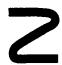
\includegraphics[keepaspectratio]{images/part002_e5542695.jpg}}

然而，\(\pi\) 作用于 T 的一个 \(\mu\) -可测子集 M 所得的像不一定是 \(\nu\) -可测的，即使 \(\pi\) 是连续的且 M 是 \(\mu\) -可忽略的（习题 7 及 §8, 习题 1）。

定理 1. --- 设 f 是定义在 X 上、取值于 \(\overline{R}\) 或一个 Banach 空间 F 中的函数。为使 f 是本质 \(\nu\) -可积的，必须且只须 \(f \circ \pi\) 是本质 \(\mu\) -可积的，此时

\[
\int \mathbf {f} (x) d \nu (x) = \int \mathbf {f} (\pi (t)) d \mu (t).\tag{3}
\]

再设 \(\pi\) 是连续且逆紧的。此时，为使 \(\mathbf{f}\) 是 \(\nu\) -可积的，必须且只须 \(\mathbf{f} \circ \pi\) 是 \(\mu\) -可积的。

只须应用 §4, No.~4 的定理 2。

推论. --- 为使 X 的一个子集 A 是本质 \(\nu\) -可积的，必须且只须 \(\overline{\pi}^{1}(A)\) 是本质 \(\mu\) -可积的，此时 \(\nu(A)=\mu\left(\overline{\pi}^{1}(A)\right)\) 。

特别地，对每个紧集 \(K \subset X\) ，\(\nu(K) = \mu\left(\overline{\pi}(K)\right)\) 。由此以及命题 2 的推论 3 推出：若 \(\mu\) 是原子的（\(\S5\) , No.~10），则 \(\pi(\mu) = \nu\) 也是原子的。因为，设 M 是由 \(t \in T\) （使 \(\mu(\{t\}) \neq 0\) 者）组成的集；由于 \(\mu\) 由 M 承载，\(\nu\) 由 \(\pi(M)\) 承载；此外，对每个 \(x \in \pi(M)\) 有 \(\nu(\{x\}) = \mu\left(\overline{\pi}(x)\right) > 0\) ，因为 \(\overline{\pi}(x)\) 至少含有 M 的一个点。因此 \(\nu\) 是原子的（\(\S5\) , No.~10, 命题 15）。

\subsection{正测度的像的性质}

命题 4. --- 设 T, T', T'' 是三个局部紧空间，μ 是 T 上的一个正测度，π 是一个由 T 到 T' 中的 μ-可测映射，π' 是一个由 T' 到 T'' 中的映射，且 π'' = π' ∘ π。

\begin{enumerate}
\def\labelenumi{\alph{enumi})}
\item
  设 \(\pi\) 是 \(\mu\) -逆紧的，并令 \(\mu' = \pi(\mu)\) 。为使 \(\pi'\) 是 \(\mu'\) -逆紧的，必须且只须 \(\pi''\) 是 \(\mu\) -逆紧的，此时 \(\pi''(\mu) = \pi'(\pi(\mu))\) （“测度的像的可迁性”）。
\item
  设 \(\pi'\) 是连续的，且 \(\pi''\) 是 \(\mu\) -逆紧的；则 \(\pi\) 是 \(\mu\) -逆紧的，\(\pi'\) 是 \(\pi(\mu)\) -逆紧的，且 \(\pi''(\mu) = \pi'(\pi(\mu))\) 。
\end{enumerate}

在 a) 的假设下，为使 \(\pi''\) 是 \(\mu\) -可测的，必须且只须 \(\pi'\) 是 \(\mu'\) -可测的（No.~2, 命题 3）。另一方面，若 K 是 \(T''\) 的一个紧子集，则 \(\pi''(K) = \pi^{-1}(\pi'(K))\) ；为使 \(\pi''(K)\) 是本质 \(\mu\) -可积的，根据定理 1 的推论，必须且只须 \(\pi'(K)\) 是本质 \(\mu'\) -可积的。最后，若 \(\pi''\) 是 \(\mu\) -逆紧的，则置 \(\mu'' = \pi''(\mu)\) ，我们对每个函数 \(f \in \mathcal{K}(T'')\) 有

\[
\begin{array}{r l} \int f (t ^ {\prime \prime}) d \mu^ {\prime \prime} (t ^ {\prime \prime}) & = \int f (\pi^ {\prime \prime} (t)) d \mu (t) \\ & = \int f (\pi^ {\prime} (\pi (t))) d \mu (t) = \int f (\pi^ {\prime} (t ^ {\prime})) d \mu^ {\prime} (t ^ {\prime}) \end{array}
\]

这是依 No.~2 的定理 1 得到的，这就完成了 a) 的证明。

在 b) 的假设下，设 \(K'\) 是 \(T'\) 的一个紧子集。则 \(K'' = \pi'(K')\) 是紧的，因此 \(\overline{\pi''}(K'')\) 是本质 \(\mu\) -可积的，从而 \(\overline{\pi}^{1}(K') \subset \overline{\pi''}(K'')\) 是本质 \(\mu\) -可积的（Ch. IV, §5, No.~5, 命题 7），于是 \(\pi\) 是 \(\mu\) -逆紧的。然后应用陈述的 a) 即完成证明。

推论. --- 设 T 和 T' 是两个局部紧空间，\(\mu\) 是 T 上的一个正测度，\(\pi\) 是一个由 T 到 T' 上的双射映射，\(\pi^{-1}\) 是逆映射。设 \(\pi\) 是 \(\mu\) -逆紧的，并令 \(\mu' = \pi(\mu)\) 。则 \(\pi^{-1}\) 是 \(\mu'\) -逆紧的，且 \(\pi^{-1}(\pi(\mu)) = \mu\) 。

命题 5. --- 设 T 和 X 是两个局部紧空间，\(\mu\) 是 T 上的一个正测度，\(\pi\) 是一个由 T 到 X 中的 \(\mu\) -逆紧映射，g 是定义在 X 上的有限数值函数 \(\geqslant 0\) ，且使得 \(g \circ \pi\) 对 \(\mu\) 局部可积。为使 g 对 \(\pi(\mu)\) 局部可积，必须且只须 \(\pi\) 对测度 \((g \circ \pi) \cdot \mu\) 是逆紧的，此时

\[
\pi \big ((g \circ \pi) \cdot \mu \big) = g \cdot \pi (\mu).\tag{4}
\]

置 \(\nu = \pi(\mu)\) 。为使 \(g\) 是局部 \(\nu\) -可积的，必须且只须 \(gf\) 是 \(\nu\) -可积的，对每个函数 \(f \in \mathcal{K}(X)\) 而言；由于 \(gf\) 具有紧支集，说 \(gf\) 是本质 \(\nu\) -可积的是同一回事，而这等价于说 \((g \circ \pi)(f \circ \pi)\) 是本质 \(\mu\) -可积的（定理 1）。但是，依 §5, No.~3 的定理 1，这表明 \(f \circ \pi\) 对 \(\rho = (g \circ \pi) \cdot \mu\) 是本质可积的，而依定义，这就是说 \(\pi\) 是 \(\rho\) -逆紧的（因为 \(\pi\) 显然是 \(\rho\) -可测的）。此外，

\[
\int f g d \nu = \int f (\pi (t)) g (\pi (t)) d \mu (t) = \int f (\pi (t)) d \rho (t)
\]

（No.~2, 定理 1 及 §5, 定理 1），这就证明了关系式 (4)。

命题 6. --- 设 T 和 X 是两个局部紧空间，\((\lambda_{\alpha})_{\alpha\in\mathbb{A}}\) 是 T 上的一个正测度族，按关系 \(\leqslant\) 有向，且在 \(\mathcal{M}(\mathrm{T})\) 中有一个上确界 \(\mu\) 。为使一个由 T 到 X 中的映射 \(\pi\) 是 \(\mu\) -逆紧的，必须且只须它是 \(\lambda_{\alpha}\) -逆紧的，对一切 \(\alpha\in A\) ，且族 \(\left(\pi(\lambda_{\alpha})\right)_{\alpha\in\mathbb{A}}\) 在 \(\mathcal{M}(\mathrm{X})\) 中有上界。此时，

\[
\pi (\mu) = \sup _ {\alpha} \pi (\lambda_ {\alpha}).\tag{5}
\]

为使 \(\pi\) 是 \(\mu\) -可测的，必须且只须 \(\pi\) 是 \(\lambda_{\alpha}\) -可测的，对一切 \(\alpha \in A\) （§1, No.~4, 命题 11 的推论 2）。设这一条件满足；说 \(\pi\) 是 \(\mu\) -逆紧的这时等价于说，对每个函数 \(f \in \mathcal{K}_{+}(X)\) ，

\[
\mu^ {\bullet} (f \circ \pi) <   + \infty .
\]

现在，

\[
\int^ {\bullet} (f \circ \pi) d \mu = \sup _ {\alpha} \int^ {\bullet} (f \circ \pi) d \lambda_ {\alpha} = \sup _ {\alpha} \int^ {\bullet} f d (\pi (\lambda_ {\alpha}))
\]

（§1, No.~4, 命题 11）；因此第一个成员对每个 \(f \in \mathcal{K}_{+}(X)\) 有限，当且仅当族 \((\pi(\lambda_{\alpha}))\) 有一个上确界 \(\theta\) （在 \(\mathcal{M}(X)\) 中），此时 \(\int(f \circ \pi) d\mu = \int f d\theta\) ，这是一个等价于 (5) 的关系式。

推论 1. --- 设 \((\mu_{\alpha})_{\alpha \in A}\) 是 T 上的一个可和的正测度族，使得 \(\mu = \sum_{\alpha \in A} \mu_{\alpha}\) ；为使一个由 T 到局部紧空间 X 中的映射 \(\pi\) 是 \(\mu\) -逆紧的，必须且只须它是 \(\mu_{\alpha}\) -逆紧的，对每个 \(\alpha \in A\) ，且族 \((\pi(\mu_{\alpha}))_{\alpha \in A}\) 是可和的。此时，

\[
\pi (\mu) = \sum_ {\alpha \in A} \pi (\mu_ {\alpha}).\tag{6}
\]

推论 2. --- 设 T 和 X 是两个局部紧空间，\((\lambda_{i})_{1\leqslant i\leqslant n}\) 是 T 上的一个有限正测度序列，并令 \(\mu=\sum_{i=1}^{n}\lambda_{i}\) 。为使一个由 T 到 X 中的映射 \(\pi\) 是 \(\mu\) -逆紧的，必须且只须它对每个指标 i 是 \(\lambda_{i}\) -逆紧的，此时

\[
\sum_ {i = 1} ^ {n} \pi (\lambda_ {i}) = \pi \left(\sum_ {i = 1} ^ {n} \lambda_ {i}\right).
\]

\subsection{复测度的像}

设 \(\theta\) 是 T 上的一个复测度，并设 \(\pi\) 是一个由 T 到局部紧空间 X 中的映射；设 \(\pi\) 是 \(\theta\) -可测的，且对每个 \(f \in \mathcal{K}(X; \mathbf{C})\) ，\(f \circ \pi\) 是本质 \(\theta\) -可积的。由于说一个函数关于 \(\theta\) 可测（相应地，本质可积）与说它关于 \(|\theta|\) 可测（相应地，本质可积）是一回事，这就表明 \(\pi\) 是 \(|\theta|\) -逆紧的。若 \(f \in \mathcal{K}(X; \mathbf{C})\) ，

\[
\left| \int (f \circ \pi) d \theta \right| \leqslant \int (| f | \circ \pi) d | \theta |;\tag{7}
\]

立即推出，线性形式 \(f \mapsto \int(f \circ \pi) d\theta\) （\(\mathcal{K}(X; \mathbf{C})\) 上的）是 X 上的一个复测度（Ch. III, §1, No.~3, 命题 6），于是可以给出下列定义：

定义 2. --- 设 \(\theta\) 是局部紧空间 T 上的一个复测度。称一个由 T 到局部紧空间 X 中的映射 \(\pi\) 为 \(\theta\) -逆紧的，如果它是 \(|\theta|\) -逆紧的。测度 \(f \mapsto \int(f \circ \pi) d\theta\) 这时称为 \(\theta\) 在 \(\pi\) 下的像，记作 \(\pi(\theta)\) 。

于是关系式 (7) 可以写成下列形式：

\[
| \pi (\theta) | \leqslant \pi (| \theta |).\tag{8}
\]

测度 \(\pi(\theta)\) 可以是零而 \(\theta\) 不是零，只要取 T 为缩成两点 a, b 的空间，取 \(\theta\) 为测度 \(\varepsilon_{a} - \varepsilon_{b}\) ，并取 \(\pi\) 为一个常值映射，即可立即看出这一点。

设 \(\theta\) 和 \(\theta'\) 是 T 上的两个复测度；若 \(\pi\) 是 \(\theta\) -逆紧的且是 \(\theta'\) -逆紧的，则由命题 6 的推论 2 推出 \(\pi\) 是 \((\theta + \theta')\) -逆紧的，因为 \(|\theta + \theta'| \leqslant |\theta| + |\theta'|\) ，且显然 \(\pi(\theta + \theta') = \pi(\theta) + \pi(\theta')\) 。

特别地，若 \(\theta\) 是一个实测度且 \(\pi\) 是 \(\theta\) -逆紧的，则

\[
\pi (\theta) = \pi (\theta^ {+}) - \pi (\theta^ {-}).\tag{9}
\]

前面建立的若干结果可以立即推广到复测度；我们列举其中最重要的。

命题 7. --- 设 \(\theta\) 是 T 上的一个复测度，\(\pi\) 是一个由 T 到局部紧空间 X 中的 \(\theta\) -逆紧映射，\(\nu\) 是像测度 \(\pi(\theta)\) 。

\begin{enumerate}
\def\labelenumi{\alph{enumi})}
\item
  设 A 是 X 的一个子集；若 \(\overline{\pi}^{1}(A)\) 是局部 \(\theta\) -可忽略的，则 A 是局部 \(\nu\) -可忽略的。
\item
  设 \(f\) 是一个由 \(X\) 到拓扑空间中的映射；若 \(f \circ \pi\) 是 \(\theta\) -可测的，则 \(f\) 是 \(\nu\) -可测的。
\item
  设 \(\mathbf{f}\) 是定义在 \(X\) 上、取值于一个 Banach 空间 \(F\) 中的函数；若 \(\mathbf{f} \circ \pi\) 是本质 \(\theta\) -可积的，则 \(\mathbf{f}\) 是本质 \(\nu\) -可积的，且
\end{enumerate}

\[
\int \mathbf {f} (\pi (t)) d \theta (t) = \int \mathbf {f} (x) d \nu (x).\tag{10}
\]

注意到公式 (8)，这些结果可由命题 2 的推论 2、命题 3 以及 No.~2 的定理 1 得出。

\subsection{应用：Lebesgue 积分中的变量替换}

设 I 是 R 的一个区间（有界或否），a 是它在 \(\overline{R}\) 中的左端点，b 是右端点，\(\mu\) 是 I 上的 Lebesgue 测度。对每个 \(\mu\) -可积函数 f 以及每个区间 \(H \subset I\) （左端点为 \(\alpha\) ，右端点为 \(\beta\) ），我们把 \(\int_{\alpha}^{\beta} \mathbf{f}(t) dt\) 写出来以代替 \(\int_{H} \mathbf{f}(t) dt = \int_{H} \mathbf{f} d\mu\) ，并置 \(\int_{\beta}^{\alpha} \mathbf{f}(t) dt = -\int_{\alpha}^{\beta} \mathbf{f}(t) dt\) ；当 f 是具有紧支集的正则函数时（Ch. IV, §4, No.~4, 例），这样赋予这些记号的意义与 FRV, II, §§1 和 2 中赋予它们的意义相一致。

设 \(g\) 是定义在 \(I\) 上且局部 \(\mu\) -可积的数值函数，\(x_0\) 是 \(I\) 的一个点；对每个 \(x \in I\) ，置

\[
G (x) = c + \int_ {x _ {0}} ^ {x} g (t) d t \quad (c \text {   a   constant }).\tag{11}
\]

数值函数 G 在 I 上连续；这由 Lebesgue 定理（Ch. IV, §4, No.~3, 定理 2 的推论 1）立即得出，因为 g 与以 x 和 \(x + h\) 为端点的区间的特征函数之积当 h 趋于 0 时趋于一个可忽略函数。因此 G(I) 是 R 的一个区间。在本 No. 中，我们把 G 看作一个由 I 到局部紧空间 G(I) 上的映射。用 \(\lambda\) 表示 I 上的测度 \(g \cdot \mu\) 。

先设 g 是 \(\mu\) -可积的。于是，与上面同样的推理表明极限 \(\mathrm{G}(a+)\) 和 \(\mathrm{G}(b-)\) 存在且有限；此外，测度 \(|\lambda|\) 是有界的（\(\S5\) , No.~3, 定理 1 的推论），且由 I 到 \(\mathrm{G}(\mathrm{I})\) 中的映射 G 是 \(\lambda\) -逆紧的。

命题 8. --- 设 g 是 \(\mu\) -可积的。若 J 表示 R 中以 \(\mathrm{G}(a+)\) 和 \(\mathrm{G}(b-)\) 为端点的开区间，则测度 \(g \cdot \mu\) 在 G 下的像是测度 \(\varphi_{J} \cdot \nu\) （若 \(\mathrm{G}(a+) \leqslant \mathrm{G}(b-)\) ）或是测度 \(-\varphi_{J} \cdot \nu\) （若 \(\mathrm{G}(a+) \geqslant \mathrm{G}(b-)\) ）（其中 \(\nu\) 表示 \(\mathrm{G}(\mathrm{I})\) 上的 Lebesgue 测度）。

只须证明，对每个函数 \(f \in \mathcal{K}\big(\mathrm{G}(\mathrm{I})\big)\) ，

\[
\int_ {\mathrm{G} (a +)} ^ {\mathrm{G} (b -)} f (\xi) d \xi = \int_ {a} ^ {b} f (\mathrm{G} (t)) g (t) d t.\tag{12}
\]

现在，这个公式对 \(g \in \mathcal{K}(\mathrm{I})\) 已经证明过了（FRV, II, §2, No.~1, 公式 (1)）。我们过渡到一般情形；存在一个序列 \((g_n)\) （由 \(\mathcal{K}(\mathrm{I})\) 中的函数组成），使得：\(1^\circ\) 序列 \((g_n(t))\) 在 I 中几乎处处趋于 \(g(t)\) ；\(2^\circ\) 存在一个 \(\mu\) -可积函数 \(h \geqslant 0\) ，使得 \(|g_n| \leqslant h\) 对一切 \(n\) 成立（Ch. IV, §3, No.~4, 定理 3）。由 Lebesgue 定理立即推出：置 \(G_n(x) = c + \int_{x_0}^x g_n(t) dt\) ，序列 \((G_n)\) 在 I 上一致收敛于 G，且数 \(G_n(a+)\) 和 \(G_n(b-)\) 分别趋于 \(G(a+)\) 和 \(G(b-)\) 。设 \(f'\) 是 \(\mathcal{K}(\mathbf{R})\) 中的一个延拓 \(f\) 的函数；上面的事实表明 \(f'(G_n(t))\) 趋于 \(f'(G(t)) = f(G(t))\) ，对一切 \(t \in \mathrm{I}\) 而言；应用 Lebesgue 定理即见公式 (12) 由公式

\[
\int_ {\mathrm{G} _ {n} (a +)} ^ {\mathrm{G} _ {n} (b -)} f ^ {\prime} (\xi) d \xi = \int_ {a} ^ {b} f ^ {\prime} \bigl (\mathrm{G} _ {n} (t) \bigr) g _ {n} (t) d t
\]

经取极限而得。

推论. --- 若一个定义在 G(I) 上、取值于 \(\overline{R}\) 或一个 Banach 空间中的函数 f 使得函数 \(t \mapsto \mathbf{f}(G(t))g(t)\) 在 I 上对 Lebesgue 测度可积，则 f 在 J 上对 Lebesgue 测度可积，且

\[
\int_ {\mathrm{G} (a +)} ^ {\mathrm{G} (b -)} \mathbf {f} (\xi) d \xi = \int_ {a} ^ {b} \mathbf {f} (\mathrm{G} (t)) g (t) d t\tag{13}
\]

（Lebesgue 积分中的变量替换公式）。

因为，\(\mathbf{f}\big(\mathrm{G}(t)\big)\) 对测度 \(|g|\cdot\mu\) 可积，从而对测度 \(g^{+}\cdot\mu\) 和 \(g^{-}\cdot\mu\) 也可积；由（No.~2 的）定理 1 推出，f 对像测度 \(\mathrm{G}(g^{+}\cdot\mu)\) 和 \(\mathrm{G}(g^{-}\cdot\mu)\) 可积，从而对测度 \(\varphi_{J}\cdot\nu\) 也可积，且 (13) 成立，这要注意到命题 8 和公式 (9)。

可能发生这样的情形：\(\mathbf{f}\) 在 J 上对 Lebesgue 测度可积，而 \(t \mapsto \mathbf{f}(\mathbf{G}(t))g(t)\) 在 I 上对 Lebesgue 测度不可积（习题 10）。

现在设 g 几乎处处保持常号（且是局部 \(\mu\) -可积的）；例如可以设 \(g(t) \geqslant 0\) 在 I 中几乎处处成立。于是 G 是 I 上的一个递增连续函数，因此 \(\mathrm{G}(a+)\) 和 \(\mathrm{G}(b-)\) 存在（但可以是无穷）。此外，G 是一个 \(\lambda\) -逆紧映射（由 I 到 \(\mathrm{G}(\mathrm{I})\) 中的）：因为，若 \(\mathrm{G}(b-) \in \mathrm{G}(\mathrm{I})\) ，则存在一个 \(x_{1} \geqslant x_{0}\) ，使得 G 对 \(x \geqslant x_{1}\) 是常值的，于是紧区间 \([G(x_{0}), G(b-)]\) 在 G 下的逆像是 \(\lambda\) -可积的；反之，若 \(G(b-) \notin G(I)\) ，则每个以 \(G(x_{0})\) 为左端点、含于 G(I) 中的紧区间在 G 下的逆像与一个紧区间至多相差一个 \(\lambda\) -可忽略区间。对以 \(G(x_{0})\) 为右端点的紧区间可类似地论证，由此得到我们的断言。此外：

命题 9. --- 设 \(g \geqslant 0\) 且局部 \(\mu\) -可积。则 \(G\) 作用于正测度 \(g \cdot \mu\) 所得的像是 \(G(I)\) 上的 Lebesgue 测度。为使一个函数 \(f\) （定义在 \(G(I)\) 上、取值于 \(\overline{R}\) 或一个 Banach 空间中）在 \(G(I)\) 上对 Lebesgue 测度可积，必须且只须函数 \(t \mapsto f(G(t))g(t)\) 在 \(I\) 上对 Lebesgue 测度可积，此时关系式 (13) 成立。

陈述的第一部分由下列事实得出：公式 (12) 对每个函数 \(f \in \mathcal{K}(\mathrm{G}(\mathrm{I}))\) 成立；因为，依上面的注记，函数 \(t \mapsto f(\mathrm{G}(t))\) 的支集含于一个区间 \(K \subset I\) ，g 在其上是可积的，只须对 K 应用命题 8。第二部分是 No.~2 的定理 1 的推论。

\subsection{切片分解。局部同胚下测度的逆像}

设 X 是一个局部紧空间，\(\pi\) 是一个由 X 到局部紧空间 T 中的映射，\(\mu\) 是 T 上的一个正测度，\(\Lambda: t \mapsto \lambda_t\) 是一个标量本质 \(\mu\) -可积且淡 \(\mu\) -可测的映射（由 T 到 \(\mathcal{M}_{+}(X)\) 中）。设 \(\nu = \int \lambda_t d\mu(t)\) 。若 \(\lambda_t\) 由 \(\overline{\pi}(t)\) 承载（对每个 \(t \in T\) ），则称等式 \(\nu = \int \lambda_t d\mu(t)\) 为 \(\nu\) 关于 \(\pi\) 的一个切片分解（或一个分解）。这一概念将在 Ch. VI 中详细研究。

命题 10. --- 沿用上述记号，设 \(\pi\) 是 \(\nu\) -可测的。设 \(g\) 是 T 上的函数 \(t \mapsto \lambda_t^*(1)\) 。为使 \(\pi\) 是 \(\nu\) -逆紧的，必须且只须 \(g\) 是局部 \(\mu\) -可积的，此时

\[
\pi (\nu) = g \cdot \mu .\tag{14}
\]

我们先在 g 局部 \(\mu\) -几乎处处有限的假设下进行论证；将在证明末尾去掉这一辅助假设。由于 \(\pi\) 依假设是 \(\nu\) -可测的，说 \(\pi\) 是 \(\nu\) -逆紧的等价于说 \(\nu^{\bullet}(f\circ\pi)<+\infty\) 对每个函数 \(f\in\mathcal{K}_{+}(\mathrm{T})\) 成立；g 既然局部几乎处处有限，我们就处于可应用 §3, No.~2 的命题 5 的断言 c) 的条件之下。因此

\[
\int^ {\bullet} (f \circ \pi) d \nu = \int^ {\bullet} d \mu (t) \int^ {\bullet} (f \circ \pi) d \lambda_ {t} = \int^ {\bullet} f (t) g (t) d \mu (t),
\]

从 \(\lambda_{t}\) 集中于 \(\overline{\pi}^{1}(t)\) 这一事实得出。我们知道 g 是 \(\mu\) -可测的，因为 \(\Lambda\) 是 \(\mu\) -适宜的（\(\S3\) , No.~1, 定义 1）。于是，说第一个成员对每个 \(f \in \mathcal{K}_{+}(\mathrm{T})\) 为有限，就等价于说 g 是局部 \(\mu\) -可积的（\(\S5\) , 命题 1），这时 (14) 由上述关系式立即得出。

于是只剩下消去辅助假设。若 g 是局部 \(\mu\) -可积的，则 g 局部 \(\mu\) -几乎处处有限，该假设确实满足。设 \(\pi\) 是 \(\nu\) -逆紧的，我们来证明 g 局部几乎处处有限。设 \(\mathfrak{K}\) 是 \(\mu\) -稠密的紧集 K（使 \(\Lambda|K\) 为淡连续者）所成之集；由于 g 可测，我们归结为证明每个紧集 \(K \in \mathfrak{K}\) （满足 \(g|K = +\infty\) ）都是 \(\mu\) -可忽略的。现设 \(\mathcal{H}\) 是函数 \(h \in \mathcal{K}_{+}(X)\) （满足 \(h \leqslant 1\) ）所成的集；置 \(g_{h}(t) = \lambda_{t}(h)\) ，用 \(\Lambda_{h}\) 表示 \(\mu\) -适宜映射 \(t \mapsto h \cdot \lambda_{t}\) ，用 \(\nu_{h}\) 表示 \(\Lambda_{h}\) 的积分，并用 f 表示 \(\mathcal{K}_{+}(T)\) 中满足 \(f \geqslant \varphi_{K}\) 的一个元素。对确实满足辅助假设的 \(\Lambda_{h}\) 应用公式 (14)，得到：

\[
\int (f \circ \pi) d \nu \geqslant \int (f \circ \pi) d \nu_ {h} = \int f g _ {h} d \mu .
\]

但函数 \(fg_h|K\) 在 \(K\) 上构成一个递增有向的连续函数集，其上包络取值 \(+\infty\) ；由 Dini 定理（GT, X, §4, No.~1, 定理 1），可以选取 \(h\) ，使得 \(fg_h|K\) 大于或等于任意一个正数 \(n\) ，由此得出 \(\int(f \circ \pi) d\nu \geqslant n \mu(K)\) 。由于 \(\pi\) 是 \(\nu\) -逆紧的，第一个成员有限，于是推出 \(\mu(K) = 0\) 。

推论 1. --- 设 \(\pi\) 是 \(\nu\) -可测的。

\begin{enumerate}
\def\labelenumi{\alph{enumi})}
\item
  若 \(\mathrm{N}\subset \mathrm{T}\) 是局部 \(\mu\) -可忽略的，则 \(\overline{\pi}^{1}(\mathrm{N})\) 是局部 \(\nu\) -可忽略的。
\item
  若 \(f\) 是一个 \(\mu\) -可测映射（由 \(T\) 到拓扑空间 \(G\) 中），则 \(f \circ \pi\) 是 \(\nu\) -可测的。
\end{enumerate}

我们重新采用前述证明末尾的记号 \(\Lambda_h\) , \(\nu_h\) , \(g_h\) ：由于 \(\nu_h\) 对每个 \(h \in \mathcal{H}\) 是有界测度，故 \(\pi\) 是 \(\nu_h\) -逆紧的，\(g_h\) 是局部 \(\mu\) -可积的，且 \(\pi(\nu_h) = g_h \cdot \mu\) 是一个以 \(\mu\) 为基的测度。由此推出，N （相应地，\(f\) ）对测度 \(\pi(\nu_h)\) 是局部可忽略的（相应地，可测的）（\(\S 5\) , No.~3, 命题 3 的推论 1 与命题 4）。因而 \(\overline{\pi}^1(N)\) （相应地，\(f \circ \pi\) ）对测度 \(\nu_h\) 是局部可忽略的（相应地，可测的）（命题 2 的推论 2，相应地为命题

3）。最后，注意到诸测度 \(\nu_{h}\) 构成一个递增有向的正测度族，其上确界为 \(\nu\) ，并应用 §1, No.~4 的命题 11 的推论 1（相应地，推论 2）。

推论 2. --- 设 \(\pi\) 是 \(\nu\) -逆紧的；设 \(\mathbf{f}\) 是定义在 \(\mathbf{T}\) 上、取值于一个 Banach 空间或 \(\overline{\mathbf{R}}\) 中的映射。为使 \(f \circ \pi\) 是本质 \(\nu\) -可积的，必须且只须 \(gf\) 是本质 \(\mu\) -可积的。

注意到命题 10，这由 §5, No.~3 的定理 1 以及 No.~2 的定理 1 立即得出。

例. --- 设 X 和 T 是两个局部紧空间，并设 \(\pi\) 是 X 到 T 中的一个局部同胚。换句话说（GT, I, §11, 习题 25），我们假设每个点 \(x \in X\) 有一个邻域 V，使得 \(\pi|V\) 是 V 到 \(\pi(x)\) 的一个邻域上的同胚；必要时把 V 换成 x 的一个相对紧开邻域 W，使得 \(\overline{W} \subset V\) ，便可推出：集 \(\mathcal{U}\) （由 X 的相对紧开子集 U 中使得 \(\pi|\overline{U}\) 是 \(\overline{U}\) 到其像上的同胚者组成）是 X 的一个开覆盖。现设 \(\mu\) 是 T 上的一个正测度；若 U 是 \(\mathcal{U}\) 的一个元素，则 \(\pi(U)\) 是紧空间 \(\pi(\overline{U})\) 中的一个开集，因而是 T 的一个局部紧子空间，并且我们知道如何定义测度 \(\mu|\pi(U)\) （由 \(\mu\) 在 \(\pi(U)\) 上诱导的）（Ch. IV, §5, No.~7）。设 \(\nu_{U}\) 是 \(\mu|\pi(U)\) 在 \(\pi|U\) 的逆同胚下的像；我们将证明存在一个且仅一个 X 上的测度 \(\nu\) ，它诱导出测度 \(\nu_{U}\) （在每个开集 \(U \in \mathcal{U}\) 上）。这个测度称为 \(\mu\) 在局部同胚 \(\pi\) 下的逆像，记作 \(\overline{\pi}^{1}(\mu)\) 。

\(\nu\) 的唯一性由局部化原理（Ch. III, §2, No.~1, 命题 1 的推论）立即得出。为建立存在性，我们注意到：若 \(t \in \mathbf{T}\) ，则每个点 \(x \in \overline{\pi}^{-1}(t)\) 有一个邻域，它与 \(\overline{\pi}^{-1}(t)\) 只交于点 \(x\) ，从而 \(\overline{\pi}^{-1}(t)\) 是 \(\mathbf{X}\) 的一个离散子空间，且族 \((\varepsilon_x)_{x \in \overline{\pi}^{-1}(t)}\) 是可和的；我们用 \(\lambda_t\) 表示它的和。接着我们证明，映射 \(t \mapsto \lambda_t\) 是标量本质 \(\mu\) -可积的，且其积分 \(\nu = \int \lambda_t d\mu(t)\) 就是所求的逆像。这将由下列引理立即得出：

引理. --- a) 设 \(f\) 是 \(\mathcal{K}_{+}(X)\) 的一个元素；函数 \(t \mapsto \lambda_{t}(f)\) 是正的、上半连续的、具有紧支集，且它在 \(\pi(X)\) 上的限制是连续的。

\begin{enumerate}
\def\labelenumi{\alph{enumi})}
\setcounter{enumi}{1}
\tightlist
\item
  设 U 是 \(\mathcal{U}\) 的一个元素，\(\nu\) 是标量本质 \(\mu\) -可积函数 \(t \mapsto \lambda_{t}\) 的积分；测度 \(\nu|U\) 在 \(\pi|U\) 下的像等于 \(\mu|\pi(U)\) 。
\end{enumerate}

为建立 a)，可借助单位分解（Ch. III, §1, No.~2, 引理 1）归结到 f 的支集 S 含于一个开集 \(U \in \mathcal{U}\) 的情形。设 g 是映射 \(t \mapsto \lambda_{t}(f)\) ；由于 \(\pi|U\) 是同胚，\(g|\pi(U)\) 属于 \(\mathcal{K}_{+}(\pi(U))\) ，于是（\((\pi(U)\) 是 \(\pi(X)\) 中的开集）g 在 \(\pi(X)\) 上的限制是连续的。由于 g 是正的且 g 在紧集 \(\pi(S)\) 上的限制连续，可见 g 在 T 上是上半连续的。由此推出 g 是 \(\mu\) -可积的。

为建立 b)，用 g 表示 \(\mathcal{K}\big(\pi(\mathrm{U})\big)\) 的一个元素，用 \(g^{\circ}\) 表示它在 T 上的以 0 延拓，用 f 表示函数 \(g \circ (\pi|U)\) ，并用 \(f^{\circ}\) 表示 f 在 X 上的以 0 延拓。断言 b) 等价于等式 \(\int g^{\circ} d\mu = \int f^{\circ} d\nu\) 。但 \(f \in \mathcal{K}(\mathrm{U})\) ，因此 \(f^{\circ} \in \mathcal{K}(\mathrm{X})\) ，于是第二个积分等于 \(\int \lambda_{t}(f^{\circ}) d\mu(t)\) 。最后 \(\lambda_{t}(f^{\circ}) = g^{\circ}(t)\) ，这就完成了证明。

现在我们注意到 \(\pi(\mathrm{X})\) 在 T 中是开集，从而是 \(\mu\) -可测的；映射 \(\Lambda: t \mapsto \lambda_t\) 是淡 \(\mu\) -可测的，因为它在 \(\pi(\mathrm{X})\) 和 \(\mathbb{C}\pi(\mathrm{X})\) 中每一个上的限制都是淡连续的。在这些条件下，公式 \(\overline{\pi}^{1}(\mu) = \int \lambda_t d\mu(t)\) 定义了 \(\overline{\pi}^{1}(\mu)\) 关于 \(\pi\) 的一个切片分解，且命题 10 给出下列结果：

命题 11. --- 设 \(\pi\) 是局部紧空间 \(X\) 到局部紧空间 \(T\) 中的一个局部同胚，设 \(\mu\) 是 \(T\) 上的一个正测度。设 \(n\) 是这样一个数值函数：它对每个 \(t \in T\) 结合 \(\overline{\pi}^{1}(t)\) 的元素个数（若此数有限），而在相反情形结合 \(+\infty\) 。为使 \(\pi\) 是 \(\overline{\pi}^{1}(\mu)\) -逆紧的，必须且只须 \(n\) 是局部 \(\mu\) -可积的，此时

\[
\pi \big (\bar {\pi} ^ {1} (\mu) \big) = n \cdot \mu .\tag{15}
\]

\section{关于诱导测度的积分}

\subsection{关于诱导测度的积分}

设 X 是 T 的一个局部紧子空间，\(\mu\) 是 T 上的一个正测度，\(\mu_{X}\) 是 \(\mu\) 在 X 上诱导的测度（Ch. IV, §5, No.~7）。对每个 \(t \in T\) ，我们用下列方式定义 X 上的一个测度 \(\lambda_{t}\) ：\(\lambda_{t} = \varepsilon_{t}\) （若 \(t \in X\) ），\(\lambda_{t} = 0\) （若 \(t \in C X\) ）。对每个定义在 X 上的有限数值函数 g，有 \(\int g(x) d\lambda_{t}(x) = g(t)\) （若 \(t \in X\) ），而 \(\int g(x) d\lambda_{t}(x) = 0\) （若 \(t \in C X\) ）。于是，若 g 是 \(\mathcal{K}(X)\) 中的一个函数，则依 \(\mu_{X}\) 的定义，我们有

\[
\mu_ {\mathrm{X}} (g) = \int \langle g, \lambda_ {t} \rangle d \mu (t).\tag{1}
\]

这就是说，可以写

\[
\mu_ {\mathrm{X}} = \int \lambda_ {t} d \mu (t)\tag{2}
\]

（§3, No.~1）。

现在让我们定义一个由 T 到 X 中的映射 \(\pi\) ：置 \(\pi(t) = t\) （对 \(t \in \mathbf{X}\) ），并置 \(\pi(t) = t_0\) （对 \(t \in \mathbb{C} \mathbf{X}\) ），其中 \(t_0\) 是 \(\mathbf{X}\) 的任意一点；可以写 \(\lambda_t = \varphi_{\mathbf{X}}(t) \varepsilon_{\pi(t)}\) ，对每个 \(t \in \mathbf{T}\) 而言。映射 \(\pi\) 是 \(\mu\) -可测的，因为它在 \(\mathbf{X}\) 和 \(\mathbb{C} \mathbf{X}\) 上的限制都是可测的（Ch. IV, §5, No.~10, 命题 16）；由此立即得出，对 \((\pi, \varphi_{\mathbf{X}})\) 是 \(\mu\) -适应的（§4, No.~1）。于是我们有下列结果：

命题 1. --- 对每个定义在 X 上的数值函数 \(g \geqslant 0\) ，

\[
\int^ {\bullet} g d \mu_ {\mathrm{X}} = \int_ {\mathrm{X}} ^ {\bullet} g d \mu\tag{3}
\]

（关于记号 \(\int_{\mathbf{X}}^{\bullet}\) ，参见 §5, No.~3, 例）。

注意到前面的注记与 (2)，关系式 (3) 由 §4 的定理 1 得出。

推论 1. --- 对 X 的每个子集 B，\(\mu_{\mathrm{X}}^{\bullet}(\mathrm{B}) = \mu^{\bullet}(\mathrm{B})\) ；为使 B 是局部 \(\mu_{\mathrm{X}}\) -可忽略的，必须且只须 B 是局部 \(\mu\) -可忽略的。

推论 2. --- 设 M 是 T 的一个子集。若 \(\mu\) 集中于 M，则 \(\mu_{X}\) 集中于 \(M \cap X\) 。

推论 3. --- 为使测度 \(\mu_{X}\) 为零，必须且只须 \(X\) 是局部 \(\mu\) -可忽略的。

注. --- 若 S 是 \(\mu\) 的支集，则 \(S \cap X\) （它在 X 中是闭的）依推论 2 包含 \(\mu_{X}\) 的支集，但可以与它不同。例如，若 \(\mu\) 是一个弥散测度而 X 是缩成一点的子空间，则诱导测度 \(\mu_{X}\) 为零，因而其支集是空的。但要注意，若 X 在 T 中是开集，则 \(\mu_{X}\) 的支集等于 \(S \cap X\) 。

命题 2. --- 为使一个由 X 到拓扑空间中的映射 g 是 \(\mu_{X}\) -可测的，必须且只须 g 在 X 中是 \(\mu\) -可测的（\(\S5\) , No.~3, 例）。

这由 §4 的命题 3 得出。

推论. --- 为使 X 的一个子集 B 是 \(\mu_{X}\) -可测的，必须且只须 B 是 \(\mu\) -可测的。

定理 1. --- 设 g 是定义在 X 上、取值于 \(\overline{R}\) 或一个 Banach 空间中的函数。为使 g 是本质 \(\mu_{X}\) -可积的，必须且只须 \(\mathbf{g}\) 在 X 中是本质 \(\mu\) -可积的（§5, No.~3, 例），此时

\[
\int \mathbf {g} d \mu_ {\mathrm{X}} = \int_ {\mathrm{X}} \mathbf {g} d \mu .\tag{4}
\]

这由 §4 的定理 2 得出。

推论 1. --- 为使 X 的一个子集 B 是本质 \(\mu_{X}\) -可积的，必须且只须它是本质 \(\mu\) -可积的，此时 \(\mu_{\mathrm{X}}(\mathrm{B}) = \mu(\mathrm{B})\) 。

推论 2. --- 设 g 是定义在 T 上且局部 \(\mu\) -可积的复值函数；则 g 在 X 上的限制 \(g_{X}\) 是局部 \(\mu_{X}\) -可积的，且

\[
(g \cdot \mu) _ {\mathrm{X}} = g _ {\mathrm{X}} \cdot \mu_ {\mathrm{X}}.\tag{5}
\]

这由定理 1（应用于诸函数 \(fg_{\mathbf{X}}\) （\(f \in \mathcal{K}(\mathbf{X}; \mathbf{C})\) ））以及复测度在 \(\mathbf{X}\) 上诱导的测度的定义（Ch. IV, §5, No.~7）立即得出。

推论 3. --- 设 \(\theta\) 是 T 上的一个复测度；则

\[
| \theta | _ {\mathrm{X}} = | \theta_ {\mathrm{X}} |.\tag{6}
\]

置 \(|\theta| = \mu\) ，并取 \(g\) 为绝对值为 1 且使 \(\theta = g \cdot \mu\) 的复值函数（§5, No.~5, 定理 2 的推论 3）而应用推论 2；则 \(\theta_{\mathrm{X}} = g_{\mathrm{X}} \cdot \mu_{\mathrm{X}}\) ；但 \(g_{\mathrm{X}}\) 是绝对值为 1 的函数，于是公式 (6) 由 §5, No.~2 的命题 2 得出。

评注. --- a) 推论 3 已用另一种方法证明过（Ch. IV, §5, No.~7, 引理 3）。

\begin{enumerate}
\def\labelenumi{\alph{enumi})}
\setcounter{enumi}{1}
\tightlist
\item
  依据推论 3，命题 1 的推论 1、2、3，命题 2，定理 1 及其推论 1、2 都可立即推广到复测度。
\end{enumerate}

概说. --- 对每个函数 \(\mathbf{f}\) （相应地，\(\mathbf{g}\) ）（定义在 X （相应地，T ）上、取值于 Banach 空间 F 或 \(\overline{\mathbf{R}}\) 中），用 \(\zeta(\mathbf{f})\) （相应地，\(\rho(\mathbf{g})\) ）表示 \(\mathbf{f}\) 到 T 上的以 0 延拓（相应地，\(\mathbf{g}\) 在 X 上的限制）。于是 \(\zeta(\rho(\mathbf{g})) = \varphi_{\mathrm{X}} \cdot \mathbf{g}\) ，\(\rho(\zeta(\mathbf{f})) = \mathbf{f}\) 。用 \(\mu'\) 表示 T 上的测度 \(\varphi_{\mathrm{X}} \cdot \mu\) 。对每个 \(p \in [1, +\infty]\) ，命题 1 与命题 2 蕴含：\(\zeta\) 把 \(\overline{\mathcal{L}}_{\mathrm{F}}^{p}(\mathrm{X}, \mu_{\mathrm{X}})\) 映入 \(\overline{\mathcal{L}}_{\mathrm{F}}^{p}(\mathrm{T}, \mu')\) ，而 \(\rho\) 把 \(\overline{\mathcal{L}}_{\mathrm{F}}^{p}(\mathrm{T}, \mu')\) 映到 \(\overline{\mathcal{L}}_{\mathrm{F}}^{p}(\mathrm{X}, \mu_{\mathrm{X}})\) 上，两种情形都保持范数，且当 \(p = 1\) 时还保持积分（定理 1）；过渡到相联系的 Hausdorff 空间，我们得到两个互为逆的同构。类似地，若把 \(\zeta\) 和 \(\rho\) 应用于正的数值函数，则本质上积分保持不变（命题 1）。这样，若约定把 X 上的函数与在 X-T 上为零的 T 上的函数等同起来，并把测度 \(\mu_{X}\) 与测度 \(\mu'\) 等同起来，则关于诱导测度的问题就归结为关于由密度定义的测度的问题，后者已在 §5 中处理。这类论证也可应用于复测度，依据定理 1 的推论 3。
